\documentclass[a4paper]{report}
\usepackage{url}
\usepackage{graphicx}
\usepackage{enumitem}
\usepackage{xcolor}
\usepackage{amsmath}
\usepackage[vlined,noresetcount]{algorithm2e}
\usepackage{tikz}
\usepackage{float}
\usepackage{amssymb}
\usepackage[dvipsnames]{xcolor}
% \usepackage{amsthm}
% \theoremstyle{definition}
% \newtheorem{definition}{Definition}[section]
\usepackage{fancyhdr}
\pagestyle{fancy}
\fancyhf{}
\fancyhead[L]{\rightmark}
\fancyhead[R]{\thepage}
\renewcommand{\headrulewidth}{0pt}

\usepackage{pgfplots} 
\pgfplotsset{width=10cm,compat=1.9}

% \usepackage{csvsimple}
% \usepackage{longtable}
\usepackage{multirow}
\usepackage{array}
\newcolumntype{L}[1]{>{\raggedright\let\newline\\\arraybackslash\hspace{0pt}}m{#1}}
\newcolumntype{C}[1]{>{\centering\let\newline\\\arraybackslash\hspace{0pt}}m{#1}}
\newcolumntype{R}[1]{>{\raggedleft\let\newline\\\arraybackslash\hspace{0pt}}m{#1}}

\makeatletter
\renewcommand{\@algocf@capt@plain}{above}% formerly {bottom}
\makeatother

\graphicspath{ {./img/} }

\begin{document}


\begin{titlepage} % Suppresses displaying the page number on the title page and the subsequent page counts as page 1
	\newcommand{\HRule}{\rule{\linewidth}{0.5mm}} % Defines a new command for horizontal lines, change thickness here
	
	\center % Centre everything on the page
	
	\includegraphics[width=7cm]{unipd_logo.png}
	\bigskip
	%------------------------------------------------
	%	Headings
	%------------------------------------------------
	
	\bigskip
	\textsc{\LARGE University of Padua}\\[1.5cm] % Main heading such as the name of your university/college
	
	\textsc{\Large }\\[0.5cm] % Major heading such as course name
	
	\textsc{\large }\\[0.5cm] % Minor heading such as course title
	
	%------------------------------------------------
	%	Title
	%------------------------------------------------
	
	\HRule\\[0.4cm]
	
	{\huge\bfseries Traveling Salesman Solver \\ Operations Research 2}\\[0.4cm] % Title of your document
	
	\HRule\\[1.5cm]
	
	%------------------------------------------------
	%	Author(s)
	%------------------------------------------------
	
	\begin{minipage}{0.4\textwidth}
		\begin{flushleft}
			\large
			\textit{Authors}\\
			Massimo Boldrin \\
            Leonardo Da Re
		\end{flushleft}
	\end{minipage}
	~
	\begin{minipage}{0.4\textwidth}
		\begin{flushright}
			\large
			\textit{Student Number}\\
			123456789 \\
            987654321
		\end{flushright}
	\end{minipage}
	
	
	\vfill\vfill\vfill % Position the date 3/4 down the remaining page
	
	{\large\today} % Date, change the \today to a set date if you want to be precise
	
	%------------------------------------------------
	%	Logo
	%------------------------------------------------
	
	%\vfill\vfill
	%\includegraphics[width=0.2\textwidth]{placeholder.jpg}\\[1cm] % Include a department/university logo - this will require the graphicx package
	 
	%----------------------------------------------------------------------------------------
	
	\vfill % Push the date up 1/4 of the remaining page
	
\end{titlepage}


\title{Traveling Salesman Problem Solver \\ Operations Research 2} % Report title

\author{Massimo Boldrin, Leonardo Da Re}

\date{\today}

\begin{abstract}
	The goal of this work is to present the Traveling Salesman Problem (TSP), a famous optimization
	problem that consists in finding the best Hamiltonian circuit on a given graph, and
	the most popular heuristics used to solve it. A presentation of these heuristics will be given, alongside an analysis of
	the performance of our implementations. Each solution is tested on a dataset of different instances, while our results are then
	compared using a customized performance profile.\\
	Firsly we briefly introduce the problem, to move into a more detailed explanation of each of the heuristics and metaheuristics used
	to solve it, to finally arrive to the algorithms that make use of the CPLEX solver from IBM.
	Additional considerations, both on the results obtained and the code decisions that we took, will be found in the last chapters.
\end{abstract}

\tableofcontents

\chapter{Introduction}

The Traveling Salesman Problem (TSP) stands as an iconic challenge in the field of combinatorial optimization, captivating researchers for its practical significance and theoretical complexity. Originating in the early 20th century, the TSP involves determining the most efficient route for a salesman to visit a set of cities exactly once before returning to the starting point. Despite its seemingly straightforward premise, the exponential growth in potential routes as cities increase presents a formidable computational challenge.

\begin{figure}[htbp]
	\centering
	\includegraphics[scale=0.15]{tsp_example}
	\caption{A solution of instance kroA150}
\end{figure}

\section{Complexity of TSP}

The Traveling Salesman Problem (TSP) is renowned not only for its practical applications but also for its classification as an NP-hard problem, signifying its computational complexity and the absence of an efficient algorithm that guarantees an optimal solution within a reasonable timeframe.

This classification as an NP-hard problem implies that as the number of cities to be visited increases, the computation required to find the optimal route escalates exponentially. The TSP's intricate nature lies in its combinatorial explosion: with n cities, the number of possible routes to consider is $(n-1)!/2$, making exhaustive exploration unfeasible for large instances. This exponential growth propels the problem into the realm of computational intractability, where conventional computing methods struggle to provide optimal solutions in a reasonable time frame.

Efforts to solve the TSP have focused on devising algorithms that offer approximate solutions or heuristics that navigate the expansive solution space more efficiently. While exact algorithms exist, such as branch-and-bound techniques, their scalability diminishes as the problem size increases. Heuristic approaches, on the other hand, aim to find near-optimal solutions within acceptable time frames by sacrificing guaranteed optimality for computational tractability.



\chapter{Coding Approaches}

\section{Approaches to Cost Function}

When talking about TSP, the distance between nodes can be seen as the cost of the edges themselves.
These type of distances are defined by TSPLIB\cite{tsplib} and can be computed or precomputed and given as input inside the .tsp files, if they are not specified to begin with.
In this project only instances where the cost of the edges is represented by the distance between nodes will be considered, hence all the instances are made of a fully connected graph.
Since the edge costs are frequently accessed during the execution of the algorithms studied in this paper, the method to retrieve them must be as fast as possible.
It is possible to differentiate between two main categories of methods for retrieving edge costs.
\newline
The first one consist in computing the distance each time it is needed, while the second method involves computing all the distances at the beginning and storing each edge value inside the memory.
While the first is the simpleset and most straightforward implementation, it does come with a major drawback: speed.
Indeed there are more than a couple distance function defined by TSPLIB, almost every instance used during this project development included the need to compute the square root at some point.
The square root operation is an operation that is computationally intesive for computers that usually require iterative algorithms to compute.
Nowadays most modern computer architectures include an hardware dedicated square root instruction, which is many times faster compared to the interative algorithm, yet still takes a lot of time to execute.
\newline
The second category of methods eliminates this problem, since allowing to compute all cost at the start completely removes the need to use any kind of cost function down the line.
On paper this method is indeed the one which allows for the greatest speedup, but, unfortunatly that is not always the case.
Since the graphs under consideration are all fully connected, the number of edges increases in a quadratic relationship to the number of nodes.
Because of this the amount of memory needed to cache the cost of all edges is in the order of $O(n^2)$, as an example 137MB of memory is needed to store the edge costs of an instance with 6000 nodes.
Although it is still a small amount of memory compared to the amount of memory modern computers are equipped with, it is too much to fit a normal personal computer CPU cache.
It's well known that CPU cache is significantly faster than regular system memory, so being unable to fit the cost matrix inside the cache can negatively impact performance.
Cache misses occur when the data the CPU needs is not found in the fast-access cache memory and must be retrieved from the slower main memory.
This delay happens because the CPU has to pause its current operations to fetch the required data, leading to increased latency and reduced overall performance.
For this reason, it is very important to access the cost matrix in a manner that is as localized as possible; otherwise, the resulting algorithm speed can be severely affected.
\figurename{ \ref{fig:matrixBadIndex}} shows the performance difference caused by swapping the row and column indices when accessing a value of the matrix.

\begin{figure}[H]
    \centering
    \begin{tikzpicture}
        \begin{axis}[
            width=11cm, height=8cm,
            ymajorgrids=true,
            grid style={dashed,gray!30},
            xlabel=Instance size,
            ymin=0, ymax=6,
            ylabel=Relative iterations/s,
            legend style={at={(0.02,0.98)},anchor=north west,legend columns=-1},
            symbolic x coords={100,500,1000,5000,10000},
            log ticks with fixed point,
            xtick=data,
            % ytick={1,2,3,4,5},
            % yticklabels={100\%,200\%,300\%,400\%,500\%},
            ybar, 
                    ]
            \addplot[Blue,fill] table[x=n, y=cmpmatrix_badindex, col sep=semicolon] {csv/cmp_2opt.csv};
            \addplot[Red,fill] table[x=n, y=cmpmatrix_goodindex, col sep=semicolon] {csv/cmp_2opt.csv};
            \legend{Bad Indexing , Good Indexing}
        \end{axis}
    \end{tikzpicture}
    \caption{Comparison between good indexing and bad indexing performance} \label{fig:matrixBadIndex}
\end{figure}

Wanting to obtain greater speed we focused on optimizing one of the method explained above.
Since the second category methods are harder to optimize, more focus was given in finding a way to compute edge cost faster, thus optimizing the first category of methods.
The lingering issue lies in the time consumed by the square root operation, which can be streamlined through various optimizations like leveraging a lookup table.
To address this, the optimization utilized SIMD instructions known as AVX.
AVX (Advanced Vector Extensions) are a set of CPU instructions designed to perform parallel operations on multiple data elements simultaneously.
They enable faster processing by allowing a single instruction to operate on multiple data points, enhancing the efficiency of tasks such as mathematical computations and data manipulation.
Supporting operations between vectors of the size of 256 bits, AVX allows computing eight distance values, in floating-point 32-bit precision, simultaneously, enhancing computational efficiency.
Another advantage is that with this approach an easy and quick approximation of the square root becomes available.
By combining the instructions for reverse square root (rsqrt) and reciprocal (rpc), it is possible to achieve an approximation with a relative error smaller than $8 \times 10^{-4}$ in less than half the time required for a precise result.
This can be leveraged by performing the initial iterations of an algorithm like 2-Opt using the approximation, then switching to exact computation once the approximation can no longer identify optimizing moves.
However, coding an algorithm to utilize AVX is more complex, and not all algorithms can be optimized this way, as they may not be suitable for vectorized execution (e.g., Simulated Annealing).

\begin{figure}[H]
    \centering
    \begin{tikzpicture}
        \begin{axis}[
            width=11cm, height=8cm,
            ymajorgrids=true,
            grid style={dashed,gray!30},
            xlabel=Instance size,
            ymin=0, ymax=0.6,
            ylabel=,
            legend style={at={(0.02,0.98)},anchor=north west,legend columns=-1},
            symbolic x coords={100,500,1000,5000,10000},
            log ticks with fixed point,
            xtick=data,
            ytick={0,0.1,0.2,0.3,0.4,0.5,0.6},
            yticklabels={0\%,10\%,20\%,30\%,40\%,50\%,60\%},
            ybar, 
                    ]
            \addplot[Red,fill] table[x=n, y=cmpavx_approx, col sep=semicolon] {csv/cmp_2opt.csv};
            %\legend{}
        \end{axis}
    \end{tikzpicture}
    \caption{Speedup percentage given by using approximated search in 2opt} \label{fig:avxApprox}
\end{figure}

\subsection{Performance Comparison}

Comparing these three approaches is complex due to numerous factors, including the number of iterations the AVX approximated method performs before switching to the exact method, and the manner in which the cost matrix is accessed.
To minimize as much as possible these external factors, the data was gathered using multiple instances sizes as well as different cost functions.
\figurename{ \ref{fig:avxShowcase}} compares all approaches, scaling the to the basic one.
As expected, using the cost matrix method is faster than the basic method for small instances but loses its advantage as instance size increases.
Throughout the entire testing, the AVX approach consistently proved to be the fastest by a significant margin in every scenario.
However, it should be noted that the AVX method yielded unstable results on smaller instances, occasionally performing slower than the matrix method.

\begin{figure}[H]
    \centering
    \begin{tikzpicture}
        \begin{axis}[
            width=11cm, height=8cm,
            ymajorgrids=true,
            grid style={dashed,gray!30},
            xlabel=Instance size,
            ymin=0, ymax=9,
            ylabel=Relative iterations/s,
            legend style={at={(0.02,0.98)},anchor=north west,legend columns=-1},
            symbolic x coords={100,500,1000,5000,10000},
            log ticks with fixed point,
            xtick=data,
            % ytick={1,2,3,4,5,6,7,8},
            % yticklabels={100\%,200\%,300\%,400\%,500\%,600\%,700\%,800\%},
            ybar, 
                    ]
            \addplot[Blue,fill] table[x=n, y=cmp_base, col sep=semicolon] {csv/cmp_2opt.csv};
            \addplot[Red,fill] table[x=n, y=cmp_matrix, col sep=semicolon] {csv/cmp_2opt.csv};
            \addplot[Green,fill] table[x=n, y=cmp_avx, col sep=semicolon] {csv/cmp_2opt.csv};
            \legend{Basic,Matrix,AVX}
        \end{axis}
    \end{tikzpicture}
    \caption{Comparison of all three approaches in 2-Opt (measurment were taken using the best optimizations found for each approach)} \label{fig:avxShowcase}
\end{figure}


\section{Multithreading}

Multithreading is a programming technique that allows a computer program to perform multiple tasks concurrently, by dividing its execution into smaller threads of execution that can run independently.
In most of the algorithms implemented, multithreading consists in running the same code on different threads while using at random different data.
This is done by means of random seed, which means, giving to each thread running a different seed value so that it may find different solutions from the other running threads.
During this process the threads share between them the globally best solution found up to that point, so that, at the end of the execution, that solution will be given as output.
This type of implementation allows to have minimal interaction between threads, allowing a great benefit in term of iterations each second as shown in \figurename{ \ref{fig:multithreadNN}}.

Although this parallel design frequently appears in algorithm implementations, it is not always feasible to use this method.
For instance, algorithms that utilize CPLEX, which is inherently designed to run on multiple threads, present such a case.
Another example is the parallelization of the 2-Opt and the 3-Opt algorithms.
As the instance size increases, both methods require progressively more time to complete their computations.
Consequently, a straightforward parallel approach was developed.
The algorithm's scalability varies based on the instance size and the number of threads used, as shown in \figurename{ \ref{fig:multithread2opt}}.

\begin{figure}[H]
    \centering
    \begin{tikzpicture}
        \begin{axis}[
            % title={Multithreading speedup of 2-Opt parallel implementation},
            xlabel={Number of Threads},
            ylabel={Iterations/s Ratio},
            xmin=1, xmax=8,
            ymin=1, ymax=8,
            xtick={1,2,3,4,5,6,7,8},%,10,12,14,16,18,20},
            ytick={1,2,3,4,5,6,7,8},%,9,10,11,12,13,14,15,16},
            legend style={at={(0.98,0.02)},anchor=south east,legend columns=1},
            ymajorgrids=true,
            xmajorgrids=true,
            grid style=dashed,
        ]
        
        \addplot[Blue,mark=square] table[x=cores, y=nn100, col sep=semicolon] {csv/MT.csv};
        \addplot[Red,mark=o] table[x=cores, y=nn1000, col sep=semicolon] {csv/MT.csv};
        \addplot[Green,mark=triangle] table[x=cores, y=nn10000, col sep=semicolon] {csv/MT.csv};
        \addlegendentry{n=100}
        \addlegendentry{n=1000}
        \addlegendentry{n=10000}
            
        \end{axis}
    \end{tikzpicture}
	\caption{Multithreading speedup of Nearest Neighbor parallel implementation} \label{fig:multithreadNN}
\end{figure}


\begin{figure}[H]
    \centering
    \begin{tikzpicture}
        \begin{axis}[
            % title={Multithreading speedup of 2-Opt parallel implementation},
            xlabel={Number of Threads},
            ylabel={Iterations/s Ratio},
            xmin=1, xmax=8,
            ymin=0, ymax=8,
            xtick={1,2,3,4,5,6,7,8},
            ytick={0,1,2,3,4,5,6,7,8},
            legend style={at={(0.02,0.98)},anchor=north west,legend columns=2},
            ymajorgrids=true,
            xmajorgrids=true,
            grid style=dashed,
        ]
        
        \addplot[SkyBlue,mark=square] table[x=cores, y=2opt100, col sep=semicolon] {csv/MT.csv};
        \addplot[Red,mark=o] table[x=cores, y=2opt500, col sep=semicolon] {csv/MT.csv};
        \addplot[Purple,mark=triangle] table[x=cores, y=2opt1000, col sep=semicolon] {csv/MT.csv};
        \addplot[Blue,mark=diamond] table[x=cores, y=2opt5000, col sep=semicolon] {csv/MT.csv};
        \addplot[Green,mark=star] table[x=cores, y=2opt10000, col sep=semicolon] {csv/MT.csv};
        \addlegendentry{n=100}
        \addlegendentry{n=500}
        \addlegendentry{n=1000}
        \addlegendentry{n=5000}
        \addlegendentry{n=10000}
            
        \end{axis}
    \end{tikzpicture}
	\caption{Multithreading speedup of 2-Opt parallel implementation} \label{fig:multithread2opt}
\end{figure}

\section{Solution Representation}

Chosing the representation for the TSP solution the memory can be a challenge since there are many ways to do so.
We chose the \textbf{Path of Indices} as our primary representation.
This method involves using a single array whose size is equal to the number of nodes.
In this array, the indices of the nodes are stored, sorted by their occurrence in the tour.
This representation offers a main advantage that we relied on: the edges in the tour can be easily determined by examining the connections between nodes in adjacent positions in the solution.
This was useful during the development of the 2-Opt and 3-Opt algorithms, since this representation implicitly represents the edges of the tour, further data structures are not necessary.
Although it must be noted that in order to make use of this advantage the most, aspecially when using the AVX approach, the first node must be attached at the end of the array as well, to represent the last visited edge in the solution.
When not working with precomputed edges cost, it is also useful to keep the coordinates X and Y of the nodes sorted to match the solution order.
This last trick allowed for a great speedup in AVX computation, since a fast \textit{load} instruction could be used as opposed to a \textit{gather} function, which generates a sequence of instructions.
A small speedup was also observed on the Basic cost computation approach, probably due to the increase in the locality of memory access which caused a reduction in the overall number of cache misses.

\subsection{Cost Cache}

Throughout our implementations, many times an array of name \textbf{Cost Cache} appears.
As its name suggests, this simple array contains the cost of each of the edges in the solution, sorted according on the order in which edges are visited in the solution.

\begin{figure}[H]
    \centering
    \begin{tikzpicture}
        \begin{axis}[
            width=11cm, height=8cm,
            ymajorgrids=true,
            grid style={dashed,gray!30},
            xlabel=Instance size,
            ymin=0, ymax=0.5,
            ylabel=,
            legend style={at={(0.02,0.98)},anchor=north west,legend columns=-1},
            symbolic x coords={100,500,1000,5000,10000},
            log ticks with fixed point,
            xtick=data,
            ytick={0,0.1,0.2,0.3,0.4},
            yticklabels={0\%,10\%,20\%,30\%,40\%},
            ybar, 
                    ]
            \addplot[Blue,fill] table[x=n, y=cmpcc_avx_cc, col sep=semicolon] {csv/cmp_2opt.csv};
            \addplot[Red,fill] table[x=n, y=cmpcc_base_cc, col sep=semicolon] {csv/cmp_2opt.csv};
            \addplot[Green,fill] table[x=n, y=cmpcc_matrix_cc, col sep=semicolon] {csv/cmp_2opt.csv};
            \legend{Basic,Matrix,AVX}
        \end{axis}
    \end{tikzpicture}
    \caption{Speedup gained by each approach using the cost cache in 2-Opt} \label{fig:costCacheShowcase} 
\end{figure}

Born at first as a simple caching method to improve the speed of some algorithms, it now serves a vital role in the Tabu Search algorithm.

\begin{figure}[H]
    \centering
    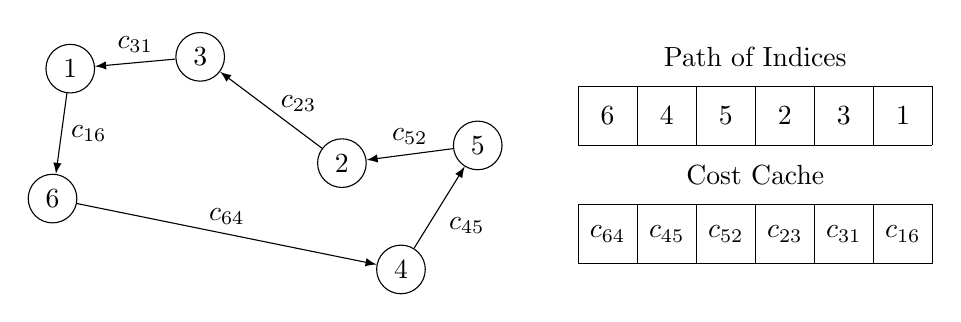
\begin{tikzpicture}[scale=0.75]
        \node[circle, draw, fill=white] (A) at (2.6, 4) {3};
        \node[circle, draw, fill=white] (B) at (0.4, 3.8) {1};
        \node[circle, draw, fill=white] (C) at (0.1, 1.6) {6};
        \node[circle, draw, fill=white] (D) at (6, 0.4) {4};
        \node[circle, draw, fill=white] (E) at (7.3, 2.5) {5};
        \node[circle, draw, fill=white] (F) at (5, 2.2) {2};
    
       \draw[-latex] (A) to node[above,] {$c_{31}$} (B);
		\draw[-latex] (B) to node[right] {$c_{16}$} (C);
		\draw[-latex] (C) to node[above] {$c_{64}$} (D);
		\draw[-latex] (D) to node[below right] {$c_{45}$} (E);
		\draw[-latex] (E) to node[above] {$c_{52}$} (F);
		\draw[-latex] (F) to node[above right, yshift=-4] {$c_{23}$} (A);
	
		\begin{scope}[shift={(9, 1.5)}]
			\draw (0,1) grid (6,2);
			\path (.5,.5) (0.5,1.5) node{$6$} ++(1,0) node{$4$} ++(1,0) node{$5$} ++(1,0) node{$2$} ++(1,0) node{$3$} ++(1,0) node{$1$};
			\draw (3,2.5) node{Path of Indices};
        \end{scope} 

		\begin{scope}[shift={(9, -0.5)}]
			\draw (0,1) grid (6,2);
			\path (.5,.5) (0.5,1.5) node{$c_{64}$} ++(1,0) node{$c_{45}$} ++(1,0) node{$c_{52}$} ++(1,0) node{$c_{23}$} ++(1,0) node{$c_{31}$} ++(1,0) node{$c_{16}$};
			\draw (3,2.5) node{Cost Cache};
        \end{scope}    

    \end{tikzpicture}
    \caption{Example of a Path of Indicies solution}
    \label{fig:solRepresentationExample}
\end{figure}

\subsection{Solution Cost Precision}

All the algorithms we implemented affect the total cost of the solution at some point, the ones that build the solution from scratch increase the cost of the tour as they iterate, while solution optimization oriented algorithm tend to decrease the overall cost by some amount at each iteration.
When used together with floating point precision, some problems might occur, especially when working on big instances;
We noticed this behavior when debugging the code of the 2-Opt algorithm:.
The earliest implementations of this algorithm in fact computed the overall cost offset of the optimization in floating point single precision (32 bits) and applied it to the overall cost which was represented as a double precision floating point (64 bits).
During the debugging phase a function to check the solution cost was called at each iteration.
That function simply followed the solution tour and increased the overall cost every time a new edge was visited.
Of course towards the end of the tour the overall cost would be much higher compared to the single edge cost that was going to be added, which means that, given a high enough instance size, the operation of computing the cost of the solution was bound to loose some precision in its representation.
This happens because of the very nature of the floating point representation.
Having said that it also stands to reason that by computing the cost the other way around would produce a ever so slightly different result.
This effect is even magnified when adding to the overall cost the cost offset value of some move, a value which is added to the sum of all the costs of the edges not, just a portion of them.
An easy fix for most of the isses caused by this precision problem is to recompute the cost of the solution each time.
The disadvantages of this fix are the fact that recomputing the cost each time is very computationally expensive, as well as the fact that the problem is not entirely solved, since the same solution cost computed backwards is not guaranteed to be the same.
We took a different approach to remove the issue entirely: we made the cost of the solution to be represented by a fixed point variable of 128 bits.
While keeping the edge costs in floating point variables, when converting to the fixed point value truncation gets rid of any possible discrepancies.
The size of 128 bits was to address a very large range of instances, since some may have nodes very close to each other which translates into small edge costs overall while other may be the opposite.
We set the separation between integer and fractional part to be in the middle, giving 64 bits for each the integer and fractional parts.

\chapter{Heuristics}

\section{Nearest Neighbor}

Nearest Neighbor (NN) is a simple, intuive and yet relatively effective greedy algorithm designed to find a feasible solution to the Traveling Salesman Problem.
This heuristic involves starting at a given point (often chosen arbitrarily or based on a specific starting condition) and then repeatedly visiting the nearest unvisited point until all points have been visited.
% In order to build the Hamiltonian circuit the algorithm indicates to move iteratively to the closest unvisited neighbor.
The key steps of the algorithm are:

\begin{enumerate}
    \item \textbf{Starting Point}: Choose an initial point (or node) as the starting location.
    \item \textbf{Nearest Neighbor Selection}: From the current point, identify the nearest unvisited point.
    \item \textbf{Move to the Nearest Point}: Travel to this nearest unvisited point.
    \item \textbf{Repeat}: Update the current point to the newly visited point and repeat the process of finding the nearest unvisited point.
    \item \textbf{Completion}: Continue until all points have been visited. In some cases, the algorithm returns to the starting point to form a complete tour (as in TSP).
    % \item select a node as starting node,
    % \item find the closes unvisited neighbor of the current node (greedy move),
    % \item move to the selected node and mark it as visited,
    % \item repeat from step 2 until all the nodes are marked as visited
\end{enumerate}

As for the initialization \textit{NN} returns a feasible solution no matter what is the starting node, but the cost of the solution will depend on it.
Therefore it is a good practice to set up a time limit and restarting the algorithm from different nodes, while keeping the best solution found so far.
While this method provides a good starting point, further refinement using a metaheuristic is usually necessary, as the initial solution is often far from optimal.
% This is due to the fact that by choosing always the closest node as the next one, it's creating a lot of crossing between edges, reducing the efficiency of the solution.

\begin{algorithm}[H]
	\TitleOfAlgo{\textbf{Nearest Neighbor}}
    \SetKwInOut{Input}{Input}
    \SetKwInOut{Output}{Output}
    \Input{
        Graph $G(V,E)$ fully connected \newline
        $c_{ij}=$ cost of $edge(i,j) \in |E|$ \newline
        Starting vertex $s$
    }
    \Output{A tour $T$ of $G$ and its cost $b$}
    \BlankLine
    $T \gets \{s\}$\\
    $v \gets s$\\
    $b \gets 0$\\
    \While{$|T| < |V|$}{
        identify $u \in V/T$ s.t. $c_{vu} \leq c_{vj}$, $\forall$ $j \in V/(T \cup {u})$\\
        $T \gets T \cup \{u\}$\\
        $b \gets b + c_{vu}$\\
        $v \gets u$\\
    }
    $b \gets b + c_{vs}$\\
    \Return $tour$, $b$\\
\end{algorithm}

\subsection{GRASP}
The above implementation of NN produces a solution which depend only on the starting node from which the algorithm starts, which means that after starting NN on all the nodes of the instance no more new solution will be found.
The \textbf{greedy randomized adaptive search procedure} (also known as \textbf{GRASP}) is a technique that allows to introduce a degree of randomization into greedy algorithms like this one.
The ways we implemented GRASP into the NN algorithm are two:
\begin{enumerate}
    \item \textit{almostbest}: 
    while searching for the nearest node, the algorithm keeps track of the $k$ nearest nodes, than using some probability one of the nodes in this list is selected.
    A simple selection method is to sort the nodes in the list from nearest to farthest and then starting from the first select it according to a probability value $p$ which is decided at the beginning.
    \item \textit{random}:
    this implementation simply adds a completely random node as successor in the solution according at any point, all according to the same probability value $p$.
\end{enumerate}
Both these enhancements have allow to run NN indefinitevly while still computing new solutions.

\subsection{Implementation}
%% ????
We have some options on how we want to run NN. First off we can decide whether to use GRASP or not, but we can also configure 
how many threads we want to use, if we want to compute the distances between points every time needed or use a matrix to store 
them, or use AVX functions when possible to improve the performances. We can also choose to use 2-opt or 3-opt after finding a 
solution to improve its cost, or we can just leave it as is.

% ######## Already in coding approaches
% By using the cost matrix to store the weight of all the edges we can speed up the computation, but this will require a tradeoff 
% in memory, O(n²) more specifically, where n is the number of nodes in the instance. Considering that we are storing nodes in a 
% matrix of float variables, this is still good for many applications, e.g. an instance of 10000 nodes will require 0.37 GB of 
% memory. This changes when we take into consideration larger instances, like the largest one in TSPlib, which includes 85900 
% nodes and would require just short of 27.5 GB of memory.
% This is why we implemented the computation of the edge weight on the fly both normally and with AVX instructions, which allows 
% us to find the solution of more complex instances.

% ????
The function that handles the application of the heuristic is NearestNeighbor, to which we pass both the instance of the 
problem and the time limit. The application of GRASP and the creation of the required number of threads is handled here.
We launch each thread with the function loopNearestNeighbor, which loops the application of applyNearestNeighbor selecting 
a different starting node every time until all nodes have been used or the time limit is reached.
At all time we keep track of the best solution found so far, which is then the one returned by NearestNeighbor. When the 
solution is return 2-opt and 3-opt will be applied as desired.

This heuristic presents two main problems: the first is that, been a greedy algorithm, at each iteration we always visit 
the next closest point and this leads to the creation of many intersection between the edges of the solution, which are 
clearly inefficient (we deal with this problem using 2-opt or 3-opt). The second one is that is a deterministic algorithm, 
which means that if we run it from the same starting node multiple times the solution will never change, so the number 
of total solutions obtainable is limited to the number of nodes.

\subsection{Performance}

Before checking how NN performs against the optimal solution it is interesting to check if there are some values of GRASP that yield a higher quality solution and which type of GRASP performs better.

\subsubsection{GRASP \textit{almostbest}}

\begin{figure}[H]
	\centering
	\begin{tikzpicture}
        \begin{axis}[
            xlabel={Cost Ratio},     % AXIS NAME
            %ylabel={Iterations/s Ratio},   % AXIS NAME
            xmin=1, xmax=1.1,       % AXIS LIMITS
            ymin=0, ymax=82,        % AXIS LIMITS
            xtick={},
            ytick=\empty,
            legend style={at={(0.98,0.02)},anchor=south east,legend columns=1}, %MOVE LEGEND HERE
			legend cell align={left},
            %ymajorgrids=true,
            xmajorgrids=true,
            grid style=dashed,
        ]
        
        \addplot[Blue,mark=square,mark size=1.5] table[x=cmp0_0.1,y=idx, col sep=semicolon] {csv/nn_almostbest.csv}; 
        \addplot[Red,mark=o,mark size=1.5] table[x=cmp0_0.05,y=idx, col sep=semicolon] {csv/nn_almostbest.csv};
        \addplot[Green,mark=triangle,mark size=1.5] table[x=cmp0_0.01,y=idx, col sep=semicolon] {csv/nn_almostbest.csv}; 
        \addlegendentry{GRASP Chance = 0.1} 
        \addlegendentry{GRASP Chance = 0.05}
        \addlegendentry{GRASP Chance = 0.01}
            
        \end{axis}
    \end{tikzpicture}
	\caption{Comparison between different grasp chances in NN with grasp type \textit{almostbest}}
    \label{fig:nnAlmostbestCmp0}
\end{figure}

From \figurename{ \ref{fig:nnAlmostbestCmp0}} it is clear that the best probability value is $0.05$.
However, by gathering more data and drawing a plot showing the relation between the best GRASP value for each instance and the size of the instances themselves, this results does not seem to be accurate.
There might be various reasons to explain these results, but lacking both the tools and the time, we did not investigate this phenomenon further.

\begin{figure}[H]
	\centering
	\begin{tikzpicture}
        \begin{axis}[
            ylabel={GRASP Chance},     % AXIS NAME
            xlabel={Number of Nodes},   % AXIS NAME
            domain=48:85901,
            ymin=0, ymax=0.15,       % AXIS LIMITS
            xmin=48, xmax=85900,        % AXIS LIMITS
            xtick={},
            ytick={0.12, 0.1, 0.085, 0.075, 0.065, 0.05, 0.03, 0.01, 0},
            yticklabel style={/pgf/number format/fixed, /pgf/number format/precision=3},
            xmode=log,
            legend style={at={(0.98,0.98)},anchor=north east,legend columns=1}, %MOVE LEGEND HERE
			legend cell align={left},
            ymajorgrids=true,
            xmajorgrids=true,
            grid style=dashed,
        ]
        
        \addplot[Red,mark=*,mark size=1, only marks] table[y=bestParam, x=n, col sep=semicolon] {csv/nn_almostbest.csv};
        \addplot[Blue,thick] plot (\x,{exp(0.68515)*\x^(-0.6464)});
        \addlegendentry{Best records} 
        \addlegendentry{Learned function}
            
        \end{axis}
    \end{tikzpicture}
	\caption{Best chance for NN GRASP type \textit{almostbest} w.r.t. the size of the instance}
    \label{fig:nnAlmostbestFunction}
\end{figure}

\begin{figure}[H]
	\centering
	\begin{tikzpicture}
        \begin{axis}[
            xlabel={Cost Ratio},     % AXIS NAME
            %ylabel={Iterations/s Ratio},   % AXIS NAME
            xmin=1, xmax=1.05,       % AXIS LIMITS
            ymin=0, ymax=82,        % AXIS LIMITS
            xtick={},
            ytick=\empty,
            legend style={at={(0.98,0.02)},anchor=south east,legend columns=1}, %MOVE LEGEND HERE
			legend cell align={left},
            %ymajorgrids=true,
            xmajorgrids=true,
            grid style=dashed,
        ]
        
        \addplot[Blue,mark=square,mark size=1.5] table[x=cmp1_0.1,y=idx, col sep=semicolon] {csv/nn_almostbest.csv}; 
        \addplot[Red,mark=o,mark size=1.5] table[x=cmp1_0.05,y=idx, col sep=semicolon] {csv/nn_almostbest.csv};
        \addplot[Green,mark=triangle,mark size=1.5] table[x=cmp1_0.01,y=idx, col sep=semicolon] {csv/nn_almostbest.csv}; 
        \addplot[Purple,mark=star,mark size=1.5] table[x=cmp1_best,y=idx, col sep=semicolon] {csv/nn_almostbest.csv}; 
        \addlegendentry{GRASP Chance = 0.1} 
        \addlegendentry{GRASP Chance = 0.05}
        \addlegendentry{GRASP Chance = 0.01}
        \addlegendentry{Dynamic GRASP Chance}
            
        \end{axis}
    \end{tikzpicture}
	\caption{Performance of the automatic chance with NN GRASP type \textit{almostbest}}
    \label{fig:nnAlmostbestCmp1}
\end{figure}

However, since we already noticed such behavior, using machine learning we fitted an exponential curve to those points obtaining the function shown in \figurename{ \ref{fig:nnAlmostbestFunction}}.
This exponential curve should actually represent the best value to use with NN and GRASP set to \textit{almostbest}, working as a \textbf{dynamic GRASP chance} w.r.t. each instance size.
After implementing this function into the code, more data was recorded and the results are displayed in \figurename{ \ref{fig:nnAlmostbestCmp1}}.

\subsubsection{GRASP \textit{random}}

Following the same idea above we discovered a similar situation.
\figurename{ \ref{fig:nnRandomFunction}} shows the best value of GRASP in \textit{random} mode, with respect to the size of each instance on which the tests were run.

\begin{figure}[H]
	\centering
	\begin{tikzpicture}
        \begin{axis}[
            ylabel={GRASP Chance},     % AXIS NAME
            xlabel={Number of Nodes},   % AXIS NAME
            domain=48:85901,
            ymin=0, ymax=0.06,       % AXIS LIMITS
            xmin=48, xmax=85900,        % AXIS LIMITS
            xtick={},
            ytick={0.05,0.03,0.02,0.01,0.005,0.001},
            xmode=log,
            legend style={at={(0.98,0.98)},anchor=north east,legend columns=1}, %MOVE LEGEND HERE
			legend cell align={left},
            ymajorgrids=true,
            xmajorgrids=true,
            grid style=dashed,
        ]
        
        \addplot[Red,mark=*,mark size=1, only marks] table[y=bestParam, x=n, col sep=semicolon] {csv/nn_random.csv};
        \addplot[Blue,thick] plot (\x,{\x^(-0.87173)});
        \addlegendentry{Best records} 
        \addlegendentry{Learned function}
            
        \end{axis}
    \end{tikzpicture}
	\caption{Best chance for NN GRASP type \textit{random} w.r.t. the size of the instance}
    \label{fig:nnRandomFunction}
\end{figure}

Again by using machine learning algorithms another exponential function was extracted from the points, this time with an overall lower value.
By gathering the necessary data using the dynamic GRASP chance we can obtrain the comparison in \figurename{ \ref{fig:nnRandomCmp1}}, which shows better performance towards the latter.

\begin{figure}[H]
	\centering
	\begin{tikzpicture}
        \begin{axis}[
            xlabel={Cost Ratio},     % AXIS NAME
            %ylabel={Iterations/s Ratio},   % AXIS NAME
            xmin=1, xmax=1.2,       % AXIS LIMITS
            ymin=0, ymax=82,        % AXIS LIMITS
            xtick={},
            ytick=\empty,
            legend style={at={(0.98,0.02)},anchor=south east,legend columns=1}, %MOVE LEGEND HERE
			legend cell align={left},
            %ymajorgrids=true,
            xmajorgrids=true,
            grid style=dashed,
        ]
        
        \addplot[Blue,mark=square,mark size=1.5] table[x=cmp_0.05,y=idx, col sep=semicolon] {csv/nn_random.csv}; 
        \addplot[Red,mark=o,mark size=1.5] table[x=cmp_0.01,y=idx, col sep=semicolon] {csv/nn_random.csv};
        \addplot[Green,mark=triangle,mark size=1.5] table[x=cmp_0.001,y=idx, col sep=semicolon] {csv/nn_random.csv}; 
        \addplot[Purple,mark=star,mark size=1.5] table[x=cmp_best,y=idx, col sep=semicolon] {csv/nn_random.csv}; 
        \addlegendentry{GRASP Chance = 0.1} 
        \addlegendentry{GRASP Chance = 0.05}
        \addlegendentry{GRASP Chance = 0.01}
        \addlegendentry{Dynamic GRASP Chance}
            
        \end{axis}
    \end{tikzpicture}
	\caption{Performance of the automatic chance with NN GRASP type \textit{random}}
    \label{fig:nnRandomCmp1}
\end{figure}

\subsubsection{NN GRASP modes comparison}

Now that the best performing parameters for each mode have been esablished, it is possible to compare all the different implementations of NN between each other. 

\begin{figure}[H]
	\centering
	\begin{tikzpicture}
        \begin{axis}[
            xlabel={Cost Ratio},     % AXIS NAME
            %ylabel={Iterations/s Ratio},   % AXIS NAME
            xmin=1, xmax=1.12,       % AXIS LIMITS
            ymin=0, ymax=82,        % AXIS LIMITS
            xtick={},
            ytick=\empty,
            legend style={at={(0.98,0.02)},anchor=south east,legend columns=1}, %MOVE LEGEND HERE
			legend cell align={left},
            %ymajorgrids=true,
            xmajorgrids=true,
            grid style=dashed,
        ]

        \addplot[Blue,mark=square,mark size=1.5] table[x=nn_cmp_nograsp,y=idxExtended, col sep=semicolon] {csv/cmp_nn_em.csv};
        \addplot[Red,mark=o,mark size=1.5] table[x=nn_cmp_almostbest,y=idxExtended, col sep=semicolon] {csv/cmp_nn_em.csv};
        \addplot[Green,mark=triangle,mark size=1.5] table[x=nn_cmp_random,y=idxExtended, col sep=semicolon] {csv/cmp_nn_em.csv};
        \addlegendentry{GRASP Disabled}
        \addlegendentry{GRASP \textit{almostbest}}
        \addlegendentry{GRASP \textit{random}}
            
        \end{axis}
    \end{tikzpicture}
	\caption{Comparison between NN GRASP modes}
    \label{fig:nnCmp}
\end{figure}

\figurename{ \ref{fig:nnCmp}} clearly shows the GRASP implementations outperforming the canonical implementation of NN by a significant amount.
While I DON'T KNOW IF I SHOULD WRITE MORE OBVIOUS STUFF ABOUT THIS.

\section{Extra Mileage}

The \textit{Extra Mileage} (EM) heuristic is another approach used to find approximate solutions to the Traveling Salesman Problem (TSP).
While similar to the Nearest Neighbor Heuristic, it comes with a slight variation in the selection process. 
In EM the idea is to minimize the additional mileage (or distance) traveled at each iteration, rather than always selecting the nearest unvisited city.
The procedure starts by creating a subtour from the instance, which can be done arbitrarily.
A subtour with just two nodes is sufficient to initiate the method.
At each iteration, we take into consideration every unvisited node in every possible position of the current subtour, and compute the increase in cost.
Let $c : V \times V \rightarrow \mathbb{R}$ be the function that, given two nodes, returns the cost of the edge between them.
Then $\forall$ covered node $i$ and uncovered node $h$: $\Delta(i,h) := $ cost of visiting $h$ right after $i$:
\[
    \Delta(i,h) = c(i,h) + c(h, succ[i]) - c(i, succ[i])
\]
We will then procede to pick the most cost-efficient option, hence, the one that increases the cost the least: $min_{i,h}\{\Delta(i,h)\}$.
The node is inserted into the correct position in the subtour, and this process continues until all nodes are marked as visited, i.e. until the tour is completed.

\begin{algorithm}[H]
	\TitleOfAlgo{\textbf{Extra Mileage}}
    \SetKwInOut{Input}{Input}
    \SetKwInOut{Output}{Output}
    \Input{
        Graph $G(V,E)$ fully connected \newline
        $c_{ij}=$ cost of $edge(i,j) \in |E|$ \newline
        Starting subtour $S$
    }
    \Output{A tour $T$ of $G$ and its cost $b$}
    \BlankLine
    $T \gets S$\\
    $b \gets$ $cost(S)$\\
    \While{{$|T| < |V|$}}{
        identify $w \in V/T$ s.t. $c_{uw} + c_{wv} - c_{uv}$ is minumum $\forall$ $u,v \in T$, $u \neq v$\\
        insert $w$ between $u$, $v$ in $T$\\
        $b \gets b + c_{uw} + c_{wv} - c_{uv}$\\
    }
    \Return $tour$, $b$\\
    
\end{algorithm}

\subsection{Implementation}
Extra mileage, like nearest neighbor, is a "solution builder", it generates a feasible solution starting from just the 
instance of the problem. Hence, we structured the implementation of this heuristic in a similar concept, maintaining the 
same configuration options, which are the application of GRASP, the number of threads to use, the computation of the edges' 
weights on the fly or store them in a matrix, and the application of 2-opt or 3-opt.

A similar structure is also implemented for the way we apply extra mileage to the instance. The main function that handles 
all the processes is ExtraMileage, which receives the instance and the time limit, sets GRASP if needed and creates the 
required number of threads.
The threads will run the function runExtraMileage until the time limit, launching in loop the function applyExtraMileage, 
which is the actual function that computes the heuristic.

\subsection{Performance}

\textbf{almostbest}

\begin{figure}[htbp]
	\centering
	\begin{tikzpicture}
        \begin{axis}[
            ylabel={GRASP Chance},     % AXIS NAME
            xlabel={Number of Nodes},   % AXIS NAME
            % domain=48:85901,
            ymin=0, ymax=0.6,       % AXIS LIMITS
            xmin=48, xmax=2393,        % AXIS LIMITS
            xtick={},
            ytick={0.5,0.4,0.3,0.2,0.15,0.1,0.05,0},
            yticklabel style={/pgf/number format/fixed, /pgf/number format/precision=4},
            xmode=log,
            legend style={at={(0.98,0.98)},anchor=north east,legend columns=1}, %MOVE LEGEND HERE
			legend cell align={left},
            ymajorgrids=true,
            xmajorgrids=true,
            grid style=dashed,
        ]
        
        \addplot[Red,mark=*,mark size=1, only marks] table[y=bestParam, x=n, col sep=semicolon] {csv/em_almostbest.csv};
        %\addplot[Blue,thick] plot (\x,{\x^(-0.87173)});
        \addlegendentry{Best records}
        %\addlegendentry{Learned function}
            
        \end{axis}
    \end{tikzpicture}
	\caption{Best chance for EM GRASP type \textit{almostbest} w.r.t. the size of the instance}
    \label{fig:emAlmostbestFunction}
\end{figure}

\begin{figure}[htbp]
	\centering
	\begin{tikzpicture}
        \begin{axis}[
            xlabel={Cost Ratio},     % AXIS NAME
            %ylabel={Iterations/s Ratio},   % AXIS NAME
            xmin=1, xmax=1.04,       % AXIS LIMITS
            ymin=0, ymax=69,        % AXIS LIMITS
            xtick={},
            ytick=\empty,
            legend style={at={(0.98,0.02)},anchor=south east,legend columns=1}, %MOVE LEGEND HERE
			legend cell align={left},
            %ymajorgrids=true,
            xmajorgrids=true,
            grid style=dashed,
        ]
        
        \addplot[Blue,mark=square,mark size=1.5] table[x=cmp_0.5,y=idx, col sep=semicolon] {csv/em_almostbest.csv}; 
        \addplot[Red,mark=o,mark size=1.5] table[x=cmp_0.3,y=idx, col sep=semicolon] {csv/em_almostbest.csv};
        \addplot[Green,mark=triangle,mark size=1.5] table[x=cmp_0.1,y=idx, col sep=semicolon] {csv/em_almostbest.csv}; 
        \addplot[Purple,mark=star,mark size=1.5] table[x=cmp_0.01,y=idx, col sep=semicolon] {csv/em_almostbest.csv}; 
        \addlegendentry{GRASP Chance = 0.5} 
        \addlegendentry{GRASP Chance = 0.3}
        \addlegendentry{GRASP Chance = 0.1}
        \addlegendentry{GRASP Chance = 0.01}
            
        \end{axis}
    \end{tikzpicture}
	\caption{Comparison of various values of chance with EM GRASP type \textit{almostbest}}
    \label{fig:emAlmostbestCmp1}
\end{figure}

\textbf{random}

\begin{figure}[htbp]
	\centering
	\begin{tikzpicture}
        \begin{axis}[
            ylabel={GRASP Chance},     % AXIS NAME
            xlabel={Number of Nodes},   % AXIS NAME
            domain=48:2393,
            ymin=0, ymax=0.11,       % AXIS LIMITS
            xmin=48, xmax=2393,        % AXIS LIMITS
            xtick={},
            ytick={0.1,0.05,0.03,0.02,0.01,0.001},
            yticklabel style={/pgf/number format/fixed, /pgf/number format/precision=3},
            xmode=log,
            legend style={at={(0.98,0.98)},anchor=north east,legend columns=1}, %MOVE LEGEND HERE
			legend cell align={left},
            ymajorgrids=true,
            xmajorgrids=true,
            grid style=dashed,
        ]
        
        \addplot[Red,mark=*,mark size=1, only marks] table[y=bestParam, x=n, col sep=semicolon] {csv/em_random.csv};
        \addplot[Blue,thick] plot (\x,{\x^(-0.97415)});
        \addlegendentry{Best records}
        \addlegendentry{Learned function}
            
        \end{axis}
    \end{tikzpicture}
	\caption{Best chance for EM GRASP type \textit{random} w.r.t. the size of the instance}
    \label{fig:emRandomFunction}
\end{figure}

\begin{figure}[htbp]
	\centering
	\begin{tikzpicture}
        \begin{axis}[
            xlabel={Cost Ratio},     % AXIS NAME
            %ylabel={Iterations/s Ratio},   % AXIS NAME
            xmin=1, xmax=1.04,       % AXIS LIMITS
            ymin=0, ymax=69,        % AXIS LIMITS
            xtick={},
            ytick=\empty,
            legend style={at={(0.98,0.02)},anchor=south east,legend columns=1}, %MOVE LEGEND HERE
			legend cell align={left},
            %ymajorgrids=true,
            xmajorgrids=true,
            grid style=dashed,
        ]
        
        \addplot[Blue,mark=square,mark size=1.5] table[x=cmp_0.03,y=idx, col sep=semicolon] {csv/em_random.csv}; 
        \addplot[Red,mark=o,mark size=1.5] table[x=cmp_0.01,y=idx, col sep=semicolon] {csv/em_random.csv};
        \addplot[Green,mark=triangle,mark size=1.5] table[x=cmp_0.001,y=idx, col sep=semicolon] {csv/em_random.csv}; 
        \addplot[Purple,mark=star,mark size=1.5] table[x=cmp_best,y=idx, col sep=semicolon] {csv/em_random.csv}; 
        \addlegendentry{GRASP Chance = 0.03} 
        \addlegendentry{GRASP Chance = 0.01}
        \addlegendentry{GRASP Chance = 0.001}
        \addlegendentry{Dynamic GRASP Chance}
            
        \end{axis}
    \end{tikzpicture}
	\caption{Comparison of various values of chance with EM GRASP type \textit{random}}
    \label{fig:emRandomCmp1}
\end{figure}

\begin{figure}[htbp]
	\centering
	\begin{tikzpicture}
        \begin{axis}[
            xlabel={Cost Ratio},     % AXIS NAME
            %ylabel={Iterations/s Ratio},   % AXIS NAME
            xmin=1, xmax=1.07,       % AXIS LIMITS
            ymin=0, ymax=69,        % AXIS LIMITS
            xtick={},
            ytick=\empty,
            legend style={at={(0.98,0.02)},anchor=south east,legend columns=1}, %MOVE LEGEND HERE
			legend cell align={left},
            %ymajorgrids=true,
            xmajorgrids=true,
            grid style=dashed,
        ]
        
        \addplot[Blue,mark=square,mark size=1.5] table[x=em_cmp_nograsp,y=idx, col sep=semicolon] {csv/cmp_nn_em.csv};
        \addplot[Red,mark=o,mark size=1.5] table[x=em_cmp_almostbest,y=idx, col sep=semicolon] {csv/cmp_nn_em.csv};
        \addplot[Green,mark=triangle,mark size=1.5] table[x=em_cmp_random,y=idx, col sep=semicolon] {csv/cmp_nn_em.csv};
        \addlegendentry{GRASP Disabled}
        \addlegendentry{GRASP \textit{almostbest}}
        \addlegendentry{GRASP \textit{random}}
            
        \end{axis}
    \end{tikzpicture}
	\caption{Comparison between EM GRASP modes}
    \label{fig:emCmp}
\end{figure}

\section{Comparison}

\begin{figure}[htbp]
	\centering
	\begin{tikzpicture}
        \begin{axis}[
            xlabel={Cost Ratio},     % AXIS NAME
            %ylabel={Iterations/s Ratio},   % AXIS NAME
            xmin=1, xmax=1.1,       % AXIS LIMITS
            ymin=0, ymax=69,        % AXIS LIMITS
            xtick={},
            ytick=\empty,
            legend style={at={(0.98,0.02)},anchor=south east,legend columns=1}, %MOVE LEGEND HERE
			legend cell align={left},
            %ymajorgrids=true,
            xmajorgrids=true,
            grid style=dashed,
        ]
        
        \addplot[Blue,mark=square,mark size=1.5] table[x=cmp_nn,y=idx, col sep=semicolon] {csv/cmp_nn_em.csv};
        \addplot[Red,mark=o,mark size=1.5] table[x=cmp_em,y=idx, col sep=semicolon] {csv/cmp_nn_em.csv};
        \addlegendentry{NN}
        \addlegendentry{EM}
            
        \end{axis}
    \end{tikzpicture}
	\caption{Comparison the quality of the output of NN and EM}
    \label{fig:cmpNNEMcost}
\end{figure}

\begin{figure}[htbp]
	\centering
	\begin{tikzpicture}
        \begin{loglogaxis}[
            xlabel={Number of nodes},     % AXIS NAME
            ylabel={Iterations/s Ratio},   % AXIS NAME
            xmin=48, xmax=2392,       % AXIS LIMITS
            ymin=1, ymax=2650,        % AXIS LIMITS
            xtick={},
            ytick={},
            legend style={at={(0.02,0.98)},anchor=north west,legend columns=1}, %MOVE LEGEND HERE
			legend cell align={left},
            %ymajorgrids=true,
            xmajorgrids=true,
            grid style=dashed,
        ]
        
        \addplot[Blue,mark=square,mark size=1.5] table[y=cmp_iters_nn, x=n, col sep=semicolon] {csv/cmp_nn_em.csv};
        \addplot[Red,mark=o,mark size=1.5] table[y=cmp_iters_em, x=n, col sep=semicolon] {csv/cmp_nn_em.csv};
        \addlegendentry{NN}
        \addlegendentry{EM}
            
        \end{loglogaxis}
    \end{tikzpicture}
	\caption{Comparison the number of iterations NN and EM were able to do within the same time limit (Probably there is no need for this figure since it can be explained by the fact that NN is $O(n^2)$ while EM is $O(n^3)$)}
    \label{fig:cmpNNEMiter}
\end{figure}


\chapter{Metaheuristics}

\section{What is a metaheuristic?}
A metaheuristic is a problem-solving strategy that consists in a set of steps, a method to be short, with the purpose of finding good solutions to optimization problems.
Unlike heuristics, they are not dependent or tailored to a specific problem in particular, instead they are general problem-solving frameworks applicable to a wide range of cases.
While heuristics are typically very specific on their execution procedure, metaheuristics usually show a higher degree of abstraction, explaining the general approach that should be followed, and leaving the actual details of the implementation to the researcher.
They do not provide guarantees on the optimality of the solution returned, but they aim to find high-quality solutions efficiently.
For this reason they often work in an iteratively manner, repeating a set of steps for a determined amount of times, until some termination condition is met.
Common termination conditions include reaching a convergence criterion in the objective function, finding a solution deemed sufficiently good, or imposing a time limit.
The broad definition of metaheuristics also accounts for the frequent need to adjust parameters for their optimization, which can differ from implementation to implementation.
%This difference with the heuristics can be confirmed also by the ones that we explored in this work. (?)
It is also noticeable that the classic version of both NN and EM are limited in discovering new solutions at each iteration, while metaheuristics usually start from an existing feasible solution, with the objective of improving it.
% Popular metaheuristics that we worked on are \textit{Simulated Annealing}, \textit{Genetic algorithm}, \textit{Tabu Search}, and \textit{Variable Neighborhood Search0}.

\section{2-Opt}
The 2-Opt metaheuristic is a local search method used to improve the solution in optimization problems.
It is based on the idea of iteratively improving a feasible solution of the problem by swapping pairs of edges creating a new solution.
Its name comes from the fact that it replaces two edges each time it optimizes the solution.
%A swap is defined as follows: given $S$ as the set of edges composing the solution and edges $e_{a,b}, e_{c,d} \in S$ a 2-Opt move consists in removing $e_{a,b}, e_{c,d}$ from $S$ and replacing them with edges $e_{a,c}, e_{b,d}$.
A \textbf{swap} is a simple computation in which two edges are removed from a feasible solution and replaced with a new pair of edges such that the solution remains feasible.
Every swap is characterized by their \textbf{offset value}, which represent the quality of the swap and is calculated as the sum of the edges added minus the sum of the edges removed.
Each solution usually allows for a a large number of swaps, however this algorithm is only interested in swaps that allows the overall cost of the tour to be reduced.
These swaps, referred to as \textbf{optimizing swaps} or \textbf{2-Opt moves}, are easily recognized by the fact that their offset is less than zero.
% \begin{definition}
%     Given a solution of TSP $S$, edge $e_1 = (a,b)$ and edge $e_2 = (c,d)$, with $e_1, e_2 \in S$ a \textbf{swap} is the substitution of $e_1$ and $e_2$ with new edges $e_3=(a,c)$ and $e_4=(b,d)$, such that $S$ remains feasible.
% \end{definition}
% Note that there exists only a single combination of edges that allows a swap output to be a feasible solution, otherwise a solution with two subtours is produced, which is an infeasible solution.
% \begin{definition}
%     A 2-Opt move between $e_1 , e_2 \in S$ and $e_3 , e_4 \notin S$ is an \textbf{optimizing swap} or \textbf{2-Opt move} \textit{iff} $C(e_3) + C(e_4) < C(e_1) + C(e_2)$ where $C(e_i)$ is the cost of edge $e_i$ and $S$ is a feasible solution.
% \end{definition}
The first step in the 2-Opt procedure consist in finding a combination of edges that allows for a 2-Opt move.
There are two main approaches to this: the first involves scanning all possible swaps and immediately performing the first 2-Opt move found, while the second involves scanning all possible swaps, identifying the best 2-Opt move, and executing it at the end.
The selected procedure is then repeated until the solution does not allow for any more optimizing swaps.

\begin{figure}[htbp]
    \centering
    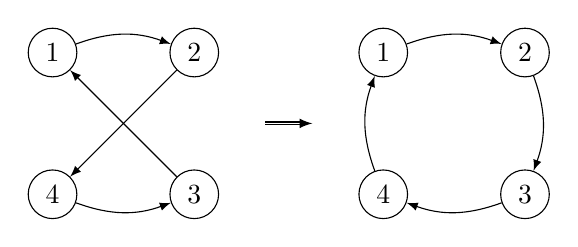
\begin{tikzpicture}[scale=0.6]
        \node[circle, draw, fill=white] (A0) at (0, 0) {1};
        \node[circle, draw, fill=white] (B0) at (3, 0) {2};
        \node[circle, draw, fill=white] (C0) at (3, -3) {3};
        \node[circle, draw, fill=white] (D0) at (0, -3) {4};
    
        \draw[-latex] (A0) to[bend left=20] (B0);
        \draw[-latex] (B0) -- (D0);
        \draw[-latex] (D0) to[bend right=20] (C0);
        \draw[-latex] (C0) -- (A0);
    
        \draw[double,-latex] (4.5,-1.5) -- (5.5,-1.5);
    
        \node[circle, draw, fill=white] (A1) at (7, 0) {1};
        \node[circle, draw, fill=white] (B1) at (10, 0) {2};
        \node[circle, draw, fill=white] (C1) at (10, -3) {3};
        \node[circle, draw, fill=white] (D1) at (7, -3) {4};
    
        \draw[-latex] (A1) to[bend left=20] (B1);
        \draw[-latex] (B1) to[bend left=20] (C1);
        \draw[-latex] (C1) to[bend left=20] (D1);
        \draw[-latex] (D1) to[bend left=20] (A1);
    \end{tikzpicture}
    \caption{2-Opt move}
    \label{fig:2optMoves}
\end{figure}

%Once the edges are swapped the total cost of the tour is recalculated, and if it is lower than the previous cost, the swap is integrated in the solution permanently, or until a better swap involving one of those two edges is found.
%This operation is iterated across all possible pairs of the tour, and is repeated until a time limit is reached, or no further improvements are possible (which involves checking all possible combinations many time, making it infeasible for real-life complex scenarios).
2-Opt can improve significantly a solution, while maintaining an acceptable computational complexity across the board.
Each iteration of 2-Opt is of $O(n^2)$ complexity, while the number of iterations depends both on the quality of the starting solution as well as on the size of the instance itself.
Its main limitation is the fact that due of it being a local search method, it may get stuck in local minima, failing to find the best solution.

\begin{figure}
    \textbf{2-Opt} \\
    \begin{algorithm}[H]
        \SetKwInOut{Input}{Input}
        % \SetKwInOut{Output}{Output}
        \Input{Graph: $G(V,E)$ \newline Cost function: $c_{ij}$ \newline A tour of $G$: $T$}
        % \Output{A better or equaly quality solution}
        \BlankLine
        $finished \gets 0$ \\
        \While{$finished = 0$}{
            $s \gets$ swap with the lowest offset currently in $T$\\
            \eIf{offset($s$) $>$ 0}{
                apply $s$ to $T$
            }{
                $finished \gets 1$
            }
        }
    \end{algorithm}
    \caption{2-Opt algorithm} \label{fig:2OptPseudocode}
\end{figure}

\subsection{Implementation}
% In our implementation of 2-opt we decided to optimize heavily the method using AVX functions rather than multithreading 
% (NOTE: check, and why AVX).
The function that takes care of the application of the metaheuristic is apply2OptBestFix, to which we pass the solution to refine, and will apply the options selected at launch. 
The heart of the algorithm lies in the two specular functions \_2OptBestFix and \_2OptBestFixApprox.
The former will compute the exact edge cost when evaluating edge swaps, considering the actual distance between the points and delivering a more precise result, with the cost of a slower computation, especially for larger instances.
The latter uses an approximated computation of the edges cost and provides a faster iteration time, with the counterpart of possibly producing slightly worse solutions. 
These two methods will iterate over all possible pairs of edges in the tour and compute the potential decrease in total tour length if we were to apply the swap.
The data regarding the best swap found so far, offset of the cost and the edges, is kept in the bestFix struct, to which we will compare each potential swap and which will be then implemented at the end of the iteration.


\subsection{3-Opt}
The 3-opt metaheuristic is an extension of 2-opt, with the difference that it no longer considers two-edge combinations but three-edge combinations instead.
This allows for a larger neighborhood of solutions, and opens to the possibility of escaping situations of local minima that 2-opt might not able to avoid.
It is worth mentioning that while the neighborhood of solutions is larger, escaping from all local minima is not guaranteed and generally not possible with algorithms such as this.
The process is mechanically the same as for 2-opt, with the main difference being the number of nodes involved in a swap and the shape those swap can take.
The concepts of \textbf{swap}, \textbf{optimizing swap} and \textbf{offset value} remain the same as they were in the 2-Opt method.
As shown in \figurename{ \ref{fig:3optMoves}}, the number of possible edge combinations increases significantly.
This, combined with the fact that the possible combinations of three edges are much more numerous than those of two edges, greatly increases computational complexity.
% As shown in figure \ref{fig:3optMoves}, starting from an existing solution, we iteratively consider three edges instead of two, and we change the way they are connected, looking for the one that has lower total cost.
% If a combination is found to improve the total cost of the solution then the swap is implemented, otherwise a different set of three edges is taken into consideration.
% Just as for 2-opt this iterative process can continue until a time limit is reached or until no more improving moves are possible.

\begin{figure}[htbp]
    \centering
    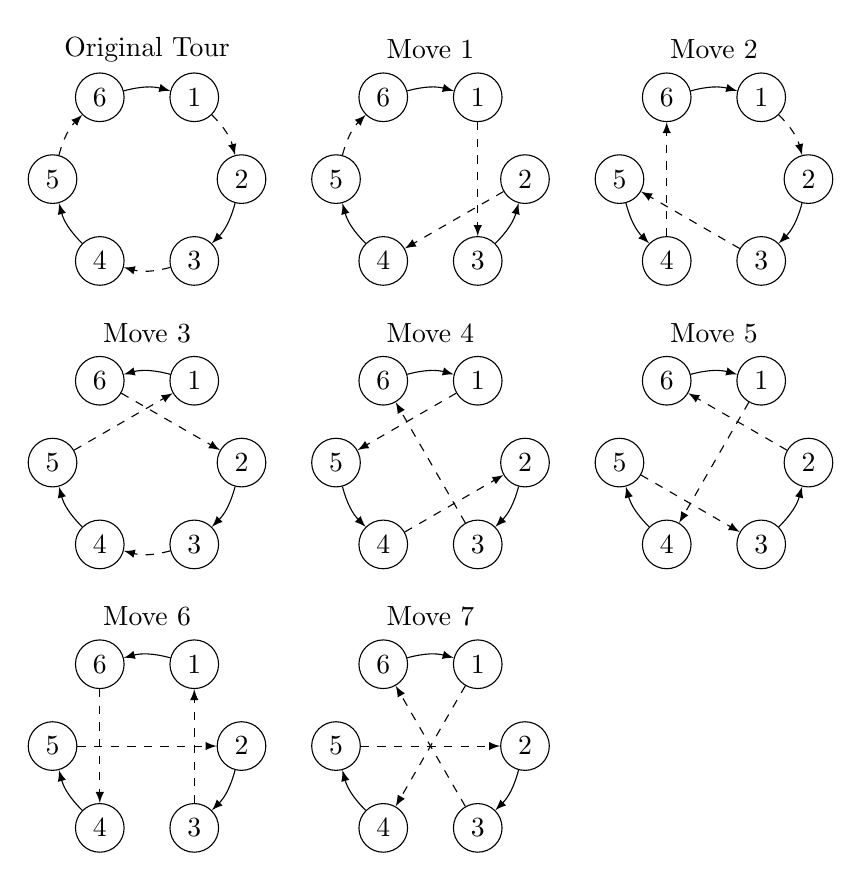
\begin{tikzpicture}[scale=0.6]
        \begin{scope}[shift={(0, 0)}]
            \node at (0, 2.75) {Original Tour};
        
            \node[circle, draw, fill=white] (N1) at ({60 * 2}:2) {6};
            \node[circle, draw, fill=white] (N2) at ({60 * 1}:2) {1};
            \node[circle, draw, fill=white] (N3) at ({60 * 0}:2) {2};
            \node[circle, draw, fill=white] (N4) at ({60 * 5}:2) {3};
            \node[circle, draw, fill=white] (N5) at ({60 * 4}:2) {4};
            \node[circle, draw, fill=white] (N6) at ({60 * 3}:2) {5};
        
            \draw[-latex] (N1) to[bend left=15] (N2);
            \draw[-latex,dashed] (N2) to[bend left=15] (N3);
            \draw[-latex] (N3) to[bend left=15] (N4);
            \draw[-latex,dashed] (N4) to[bend left=15] (N5);
            \draw[-latex] (N5) to[bend left=15] (N6);
            \draw[-latex,dashed] (N6) to[bend left=15] (N1);
        \end{scope}
    
        \begin{scope}[shift={(6, 0)}]
            \node at (0, 2.75) {Move 1};
        
            \node[circle, draw, fill=white] (N1) at ({60 * 2}:2) {6};
            \node[circle, draw, fill=white] (N2) at ({60 * 1}:2) {1};
            \node[circle, draw, fill=white] (N3) at ({60 * 0}:2) {2};
            \node[circle, draw, fill=white] (N4) at ({60 * 5}:2) {3};
            \node[circle, draw, fill=white] (N5) at ({60 * 4}:2) {4};
            \node[circle, draw, fill=white] (N6) at ({60 * 3}:2) {5};
        
            \draw[-latex] (N1) to[bend left=15] (N2);
            \draw[-latex,dashed] (N2) to (N4);
            \draw[-latex,dashed] (N3) to (N5);
            \draw[-latex] (N4) to[bend right=15] (N3);
            \draw[-latex] (N5) to[bend left=15] (N6);
            \draw[-latex,dashed] (N6) to[bend left=15] (N1);
        \end{scope}
    
        \begin{scope}[shift={(12, 0)}]
            \node at (0, 2.75) {Move 2};
        
            \node[circle, draw, fill=white] (N1) at ({60 * 2}:2) {6};
            \node[circle, draw, fill=white] (N2) at ({60 * 1}:2) {1};
            \node[circle, draw, fill=white] (N3) at ({60 * 0}:2) {2};
            \node[circle, draw, fill=white] (N4) at ({60 * 5}:2) {3};
            \node[circle, draw, fill=white] (N5) at ({60 * 4}:2) {4};
            \node[circle, draw, fill=white] (N6) at ({60 * 3}:2) {5};
        
            \draw[-latex] (N1) to[bend left=15] (N2);
            \draw[-latex,dashed] (N2) to[bend left=15] (N3);
            \draw[-latex] (N3) to[bend left=15] (N4);
            \draw[-latex,dashed] (N4) to (N6);
            \draw[-latex,dashed] (N5) to (N1);
            \draw[-latex] (N6) to[bend right=15] (N5);
        \end{scope}
    
        \begin{scope}[shift={(0, -6)}]
            \node at (0, 2.75) {Move 3};
        
            \node[circle, draw, fill=white] (N1) at ({60 * 2}:2) {6};
            \node[circle, draw, fill=white] (N2) at ({60 * 1}:2) {1};
            \node[circle, draw, fill=white] (N3) at ({60 * 0}:2) {2};
            \node[circle, draw, fill=white] (N4) at ({60 * 5}:2) {3};
            \node[circle, draw, fill=white] (N5) at ({60 * 4}:2) {4};
            \node[circle, draw, fill=white] (N6) at ({60 * 3}:2) {5};
        
            \draw[-latex,dashed] (N1) to (N3);
            \draw[-latex] (N2) to[bend right=15] (N1);
            \draw[-latex] (N3) to[bend left=15] (N4);
            \draw[-latex,dashed] (N4) to[bend left=15] (N5);
            \draw[-latex] (N5) to[bend left=15] (N6);
            \draw[-latex,dashed] (N6) to (N2);
        \end{scope}
    
        \begin{scope}[shift={(6, -6)}]
            \node at (0, 2.75) {Move 4};
        
            \node[circle, draw, fill=white] (N1) at ({60 * 2}:2) {6};
            \node[circle, draw, fill=white] (N2) at ({60 * 1}:2) {1};
            \node[circle, draw, fill=white] (N3) at ({60 * 0}:2) {2};
            \node[circle, draw, fill=white] (N4) at ({60 * 5}:2) {3};
            \node[circle, draw, fill=white] (N5) at ({60 * 4}:2) {4};
            \node[circle, draw, fill=white] (N6) at ({60 * 3}:2) {5};
        
            \draw[-latex] (N1) to[bend left=15] (N2);
            \draw[-latex,dashed] (N2) to (N6);
            \draw[-latex] (N3) to[bend left=15] (N4);
            \draw[-latex,dashed] (N4) to (N1);
            \draw[-latex,dashed] (N5) to (N3);
            \draw[-latex] (N6) to[bend right=15] (N5);
        \end{scope}
    
        \begin{scope}[shift={(12, -6)}]
            \node at (0, 2.75) {Move 5};
        
            \node[circle, draw, fill=white] (N1) at ({60 * 2}:2) {6};
            \node[circle, draw, fill=white] (N2) at ({60 * 1}:2) {1};
            \node[circle, draw, fill=white] (N3) at ({60 * 0}:2) {2};
            \node[circle, draw, fill=white] (N4) at ({60 * 5}:2) {3};
            \node[circle, draw, fill=white] (N5) at ({60 * 4}:2) {4};
            \node[circle, draw, fill=white] (N6) at ({60 * 3}:2) {5};
        
            \draw[-latex] (N1) to[bend left=15] (N2);
            \draw[-latex,dashed] (N2) to (N5);
            \draw[-latex,dashed] (N3) to (N1);
            \draw[-latex] (N4) to[bend right=15] (N3);
            \draw[-latex] (N5) to[bend left=15] (N6);
            \draw[-latex,dashed] (N6) to (N4);
        \end{scope}
    
        \begin{scope}[shift={(0, -12)}]
            \node at (0, 2.75) {Move 6};
        
            \node[circle, draw, fill=white] (N1) at ({60 * 2}:2) {6};
            \node[circle, draw, fill=white] (N2) at ({60 * 1}:2) {1};
            \node[circle, draw, fill=white] (N3) at ({60 * 0}:2) {2};
            \node[circle, draw, fill=white] (N4) at ({60 * 5}:2) {3};
            \node[circle, draw, fill=white] (N5) at ({60 * 4}:2) {4};
            \node[circle, draw, fill=white] (N6) at ({60 * 3}:2) {5};
        
            \draw[-latex,dashed] (N1) to (N5);
            \draw[-latex] (N2) to[bend right=15] (N1);
            \draw[-latex] (N3) to[bend left=15] (N4);
            \draw[-latex,dashed] (N4) to (N2);
            \draw[-latex] (N5) to[bend left=15] (N6);
            \draw[-latex,dashed] (N6) to (N3);
        \end{scope}
    
        \begin{scope}[shift={(6, -12)}]
            \node at (0, 2.75) {Move 7};
        
            \node[circle, draw, fill=white] (N1) at ({60 * 2}:2) {6};
            \node[circle, draw, fill=white] (N2) at ({60 * 1}:2) {1};
            \node[circle, draw, fill=white] (N3) at ({60 * 0}:2) {2};
            \node[circle, draw, fill=white] (N4) at ({60 * 5}:2) {3};
            \node[circle, draw, fill=white] (N5) at ({60 * 4}:2) {4};
            \node[circle, draw, fill=white] (N6) at ({60 * 3}:2) {5};
        
            \draw[-latex] (N1) to[bend left=15] (N2);
            \draw[-latex,dashed] (N2) to (N5);
            \draw[-latex] (N3) to[bend left=15] (N4);
            \draw[-latex,dashed] (N4) to (N1);
            \draw[-latex] (N5) to[bend left=15] (N6);
            \draw[-latex,dashed] (N6) to (N3);
        \end{scope}
    
    \end{tikzpicture}
    \caption{3-Opt available moves}
    \label{fig:3optMoves}
\end{figure}

\section{Tabu Search}
Tabu search is a metaheuristic that focuses on escaping local minima.
The idea is to avoid solutions that we know that cannot lead to the global optima.
Let's assume that we alredy have a refined solution, and that we have reached a local minima using the 2-Opt algorithm, let's call this solution $x_i$. 
Trying to further refine it will not provide any improvement, since $x_i$ does not contain any optimizing swap because it was obtained using 2-Opt.
The approach Tabu Search uses to escape from this situation is that of accepting a \textit{bad} move, in other words it performs a swap even if it will cause the cost of the overall cost of the tour to increase.
Therefore a new tour is produced, $x_j$, in the hope that applying 2-Opt once again will yield better solution then $x_i$.
% Hence, the only way to move from this neighborhood of solutions is to accept a \textit{bad} move, in other words we need to perform a swap of some edges that will worsen the solution, generating a new one called $x_{k+1}$, in the hope from it we will be  able to reach a better one.
However there is a high chance that the local search algorithm will turn back from $x_j$ to $x_i$, thus nullifying all the previous efforts.
To avoid this Tabu Seach implements a list called \textbf{tenure} which contains those swaps that are done to escape a local minima.
The tenure works as a list of \textit{forbidden moves} which means that 2-Opt will not be able to perform swaps included within this data structure.
%The way that Tabu Search does this is by implementing a list of edges that cannot be touched, called \textbf{tenure}.
% Any of the edges in this list are \textit{fixed} and we are not allowed to move them with a 2-opt-type move, which forbids a backwards movement from $x_{k+1}$ to $x_k$.
% Logically, without this list, if we were to perform a swap that worsens the solution and we were to  apply 2-opt right after we would just go back to $x_k$, which is the local minima we are trying to escape from.
Of course there are some other considerations to be done on the tenure, involving its size as well as its contents.
Intuitively, the size of this list should be limited, otherwise it might block too many edges and the optimization will become stuck regardless.
Once the list is full, newly introduced \textit{forbidden moves} replace the oldest element in the tenure. 
Another potential improvements regards a detection mechanism on whether the local minima has been escaped or not: by checking if 2-Opt made any improvements on the solution, even while avoiding \textit{forbidden moves}, it is possible to have a rough estimation on wether or not the local optima point has been escaped or not.
Upon detecting a potential escape, removing the oldest element from the tenure in hope of having actually escaped of the local minima.
% This size is called \textit{NOT TENURE}, and could be a fixed amount or it could be adaptive depending on the instance of the problem we are approaching.
% When the list is full, we start replacing the edges in it starting from the older ones.
It is imperative for this procedure to work to its fullest to always keep a copy of the best solution found throughout its execution at all times.
As for the other metaheuristic presented, this process can continue until some termination condition is reached.

\subsection{Implementation(? Maybe talk about the edge locking mechanism)}
TabuSearch is the main method that manages the execution of the tabu algorithm.
After receiving the solution, it sets the tenure size, which is implemented as an array of struct Edge, accordingly to input.
We implemented a check on the value passed for this parameter: if we don't receive any specific size the default value of 2 is set; if we receive a value that is larger of equal to the amount of nodes in 
the instace an error is thrown, since this will lead to the algorithm getting stuck; and lastly, if the value is larger than the 97\% of the 
number of nodes a warning message will indicate the possibility of the method getting stuck and not respecting the time limit.
After this, the function runTabu is launched whithin the threads and takes care of the execution of the metaheuristic, starting from the current best solution (CHECK IF ITS THE PASSED SOLUTION).
The main loop that keeps going until the time limit consists in selecting two random edges in the solution, swapping them and locking one of the two by inserting it into the tenure.
Once we have done that 2-opt is launched to refine the solution, and we keep relaunching it until there are no further improving moves possible, freeing the oldest element in the tenure before relaunching it every time.
A counter is implemented to keep track of the number of iteration in which the method does not find a solution 
that is better than the best one found so far, and when it reaches a threshold the working solution of the thread is resetted back to the best one.

\subsection{Performance}

\begin{figure}[H]
	\centering
	\begin{tikzpicture}
        \begin{axis}[
            xlabel={Cost Ratio},     % AXIS NAME
            %ylabel={Iterations/s Ratio},   % AXIS NAME
            xmin=1, xmax=1.03,       % AXIS LIMITS
            ymin=0, ymax=74,        % AXIS LIMITS
            xtick={},
            ytick=\empty,
            legend style={at={(0.98,0.02)},anchor=south east,legend columns=1}, %MOVE LEGEND HERE
			legend cell align={left},
            %ymajorgrids=true,
            xmajorgrids=true,
            grid style=dashed,
        ]
        
        \addplot[Blue,mark=square,mark size=1.5] table[x=p1cost,y=idx, col sep=semicolon] {csv/tabu.csv}; 
        \addplot[Red,mark=o,mark size=1.5] table[x=p2cost,y=idx, col sep=semicolon] {csv/tabu.csv};
        \addplot[Green,mark=triangle,mark size=1.5] table[x=p3cost,y=idx, col sep=semicolon] {csv/tabu.csv}; 
        \addlegendentry{Tenure size = 1} 
        \addlegendentry{Tenure size = 2}
        \addlegendentry{Tenure size = 3}
            
        \end{axis}
    \end{tikzpicture}
	\caption{Performance comparison between different tenure sizes \label{fig:tabuParmTune}}
\end{figure}

\begin{figure}[H]
	\centering
	\begin{tikzpicture}
        \begin{axis}[
            xlabel={Cost Ratio},     % AXIS NAME
            %ylabel={Iterations/s Ratio},   % AXIS NAME
            xmin=1, xmax=1.082,       % AXIS LIMITS
            ymin=0, ymax=74,        % AXIS LIMITS
            xtick={},
            ytick=\empty,
            legend style={at={(0.98,0.02)},anchor=south east,legend columns=1}, %MOVE LEGEND HERE
			legend cell align={left},
            %ymajorgrids=true,
            xmajorgrids=true,
            grid style=dashed,
        ]
        
        \addplot[Blue,mark=square,mark size=1.5] table[x=startcost,y=idx, col sep=semicolon] {csv/tabu.csv}; 
        \addplot[Red,mark=o,mark size=1.5] table[x=finalcost,y=idx, col sep=semicolon] {csv/tabu.csv};
        \addplot[Green,mark=triangle,mark size=1.5] table[x=optimalcost,y=idx, col sep=semicolon] {csv/tabu.csv}; 
        \addlegendentry{Initial Cost} 
        \addlegendentry{Final Cost}
        \addlegendentry{Optimal Cost}
            
        \end{axis}
    \end{tikzpicture}
	\caption{Performance of with tenure size set to 1 \label{fig:tabuCost}}
\end{figure}

\begin{figure}[H]
	\centering
	\begin{tikzpicture}
        \begin{axis}[
            ylabel={Iterations/s Ratio},     % AXIS NAME
            xlabel={Sorted instances},   % AXIS NAME
            xmin=0, xmax=74,       % AXIS LIMITS
            ymin=1, ymax=1.1,        % AXIS LIMITS
            ytick={},
            xtick=\empty,
            legend style={at={(0.02,0.98)},anchor=north west,,legend columns=1}, %MOVE LEGEND HERE
			legend cell align={left},
            ymajorgrids=true,
            %xmajorgrids=true,
            grid style=dashed,
        ]
        
        \addplot[Blue,mark=square,mark size=1.5] table[y=p1iter,x=idx, col sep=semicolon] {csv/tabu.csv};
        \addplot[Red,mark=o,mark size=1.5] table[y=p2iter,x=idx, col sep=semicolon] {csv/tabu.csv};
        \addplot[Green,mark=triangle,mark size=1.5] table[y=p3iter,x=idx, col sep=semicolon] {csv/tabu.csv};
        \addlegendentry{Tenure size = 1}
        \addlegendentry{Tenure size = 2}
        \addlegendentry{Tenure size = 3} 
            
        \end{axis}
    \end{tikzpicture}
	\caption{Comparison between tabu search parameters and iteration count \label{fig:tabuIters}}
\end{figure}

\section{Variable Neighborhood Search}

Variable Neighborhood Search (VNS) is a technique that explores various neighborhoods within the solution space to seek a potentially optimal solution to a problem.
This metaheuristic closely resembles Tabu Search at a high level of abstraction.
It begins with a feasible solution and explores its neighborhood to identify the best solution within that vicinity before moving on to another neighborhood.
The aim of VNS is to explore different portions of the solution space with the hope of eventually finding the neighborhood of the optimal solution.
% After that we move onto another neighborhood and we explore that one.
The differnce with the previous algorithm is in its behavior on incurring into local minima.
Instead of executing a move that necessarily worsens the solution, VNS addresses the problem by making a completely random move, informally referred to as "kick".
% Indeed there are many type of moves that are suitable for this algorithm, the one we implemented works as follows:
% using $n$ as the magnitude of the "kick", 

While we do this process we keep track of the best solution found so far, and we replace it when a new neighborhood reveals a better minima.
In TSP, to explore the neighborhood of a solution we can use local search algorithms like 2-opt and 3-opt, while to change the neighborhood we perform a swap on a higher amout of edges, five, for instance.
Doing this allows us change the space in which we search for the solution using local search maintaining most of the existing tour untouched.

\begin{figure}[htbp]
    \centering
    \begin{tikzpicture}[scale=1]
        \draw[->] (0,0) -- node[below] {Solution Space} (11,0);
        \draw[->] (0,0) -- node[above,sloped] {Cost} (0,9);
    
        \coordinate (A) at (1, 7);
        \coordinate (B) at (2, 7.5);
        \coordinate (C) at (3, 5);
        \coordinate (D) at (4, 6);
        \coordinate (E) at (5, 3.5);
        \coordinate (F) at (6, 5);
        \coordinate (G) at (7, 1);
        \coordinate (H) at (8, 3.5);
        \coordinate (I) at (9, 4);
        \coordinate (J) at (10, 3.5);
    
        \draw[black,thick] plot [smooth] coordinates {(A) (B) (C) (D) (E) (F) (G) (H) (I) (J)};
    
        \coordinate (P1) at (2.08,7.4);
        \coordinate (P2) at (3.07,5.01);
        \coordinate (P3) at (4.18,5.7);
        \coordinate (P4) at (5.02,3.52);
        \coordinate (P5) at (6.07,4.9);
        \coordinate (P6) at (7.04,1.02);
        
        % Draw jump arrows
        \draw[black,-latex] ([yshift=4]P2) to[out=90, in=180] (3.82,6.4) to[out=0, in=90] ([yshift=4]P3);
        \node[above] at (3.75,6.4) {kick};
        \draw[black,-latex] ([yshift=4]P4) to[out=90, in=180] (5.75,5.5) to[out=0, in=90] ([yshift=4]P5);
        \node[above] at  (5.65,5.5) {kick};
        
        % Comment arrows
        \draw[black,-latex] (2.5,8) -- ([xshift=2,yshift=3.6]P1);
        \node[above right,yshift=0,text width=25mm] at (2.5,8) {\quad Starting \quad Configuration};
        \draw[black,-latex] (6,1) -- ([xshift=-4,yshift=-0.6]P6);
        \node[left,xshift=13,yshift=0,text width=18mm] at (6,1) {\ Global \ Minimum};
        
    
        % Draw points
        \foreach \point in {P1,P2,P3,P4,P5,P6}  {
            \filldraw [black] (\point) circle (2.5pt);
            \filldraw [cyan] (\point) circle (2pt);
        }
    
    \end{tikzpicture}
    \caption{Iteration process of VNS}
    \label{fig:vns}
\end{figure}

VNS balances exploration (through varying neighborhood structures) and exploitation (through local search) to efficiently search the solution space.
The number of edges that we decide to swap can be dependent of the size of the instance, if we were working on a small instance, e.g. 
~50 nodes, swapping more than ten edges could result in a change way too big of the starting solution, worsening it unnecessarily.

\subsection{Implementation(? Maybe talk specifics on how kick works)}
For the implementation of VNS we have the main function VariableNeighborhoodSearch which is in charge of managing the various threads initialization 
and coordination, along with the time management in order to maintain the execution of the algorithm within the time limit provided in input.
Inside the threads we will run parallely the function runVns, which performs the actual algorithm.
The loop inside the threads will start by taking the passed solution and perform a repeating cycle of 2-opt operations and kicks. 2-opt is in charge 
of searching the local space of the solution, while the kick will ensure a traslation to a neighboring search space.
For the kick we implemented a swap of a dynamically chosen amount of edges. We did this to adapt to different scales of instances, since a fixed 
amount of edges swaps (e.g. five each time) could result in a non-effective enough of a neighborhood change for large instances. All the edges involved in the kick are selected randomly.
After each execution of 2-opt the obtained solution will be compared with the saved best solution found so far, and, if the cost is improved, the 
best solution gets updated. Note that the best solution is shared among the threads and its access is managed by mutex.

\subsection{Performance}

\begin{figure}[H]
	\centering
	\begin{tikzpicture}
        \begin{axis}[
            xlabel={Cost Ratio},     % AXIS NAME
            %ylabel={Iterations/s Ratio},   % AXIS NAME
            xmin=1, xmax=1.015,       % AXIS LIMITS
            ymin=0, ymax=74,        % AXIS LIMITS
            xtick={1,1.005,1.01,1.015},
            xticklabel style={/pgf/number format/fixed,/pgf/number format/precision=4},
            ytick=\empty,
            legend style={at={(0.98,0.02)},anchor=south east,legend columns=1}, %MOVE LEGEND HERE
			legend cell align={left},
            %ymajorgrids=true,
            xmajorgrids=true,
            grid style=dashed,
        ]
        
        \addplot[Blue,mark=square,mark size=1.5] table[x=p4_4cost, y=idx, col sep=semicolon] {csv/vns.csv}; 
        \addplot[Red,mark=o,mark size=1.5] table[x=p5_5cost, y=idx, col sep=semicolon] {csv/vns.csv};
        \addplot[Green,mark=triangle,mark size=1.5] table[x=p5_10cost, y=idx, col sep=semicolon] {csv/vns.csv};
        \addplot[Purple,mark=star,mark size=1.5] table[x=p5_20cost, y=idx, col sep=semicolon] {csv/vns.csv};
        \addplot[Dandelion,mark=otimes,mark size=1.5] table[x=p5_40cost, y=idx, col sep=semicolon] {csv/vns.csv};
        \addplot[Black,mark=diamond,mark size=1.5] table[x=p20_40cost, y=idx, col sep=semicolon] {csv/vns.csv};
        \addlegendentry{Kick Config = (4,4)}
        \addlegendentry{Kick Config = (5,5)}
        \addlegendentry{Kick Config = (5,10)}
        \addlegendentry{Kick Config = (5,20)}
        \addlegendentry{Kick Config = (5,40)}
        \addlegendentry{Kick Config = (20,40)}
            
        \end{axis}
    \end{tikzpicture}
	\caption{Performance comparison between different KICKs configurations \label{fig:vnsParmTune}}
\end{figure}

\begin{figure}[H]
	\centering
	\begin{tikzpicture}
        \begin{axis}[
            xlabel={Cost Ratio},     % AXIS NAME
            %ylabel={Iterations/s Ratio},   % AXIS NAME
            xmin=1, xmax=1.082,       % AXIS LIMITS
            ymin=0, ymax=74,        % AXIS LIMITS
            xtick={},
            ytick=\empty,
            legend style={at={(0.98,0.02)},anchor=south east,legend columns=1}, %MOVE LEGEND HERE
			legend cell align={left},
            %ymajorgrids=true,
            xmajorgrids=true,
            grid style=dashed,
        ]
        
        \addplot[Blue,mark=square,mark size=1.5] table[x=startcost,y=idx, col sep=semicolon] {csv/vns.csv}; 
        \addplot[Red,mark=o,mark size=1.5] table[x=finalcost,y=idx, col sep=semicolon] {csv/vns.csv};
        \addplot[Green,mark=triangle,mark size=1.5] table[x=optimalcost,y=idx, col sep=semicolon] {csv/vns.csv}; 
        \addlegendentry{Initial Cost} 
        \addlegendentry{Final Cost}
        \addlegendentry{Optimal Cost}
            
        \end{axis}
    \end{tikzpicture}
	\caption{Performance of with KICK configuration set to (5,10) \label{fig:vnsCost}}
\end{figure}

\begin{figure}[H]
	\centering
	\begin{tikzpicture}
        \begin{axis}[
            ylabel={Iterations/s Ratio},     % AXIS NAME
            xlabel={Sorted instances},   % AXIS NAME
            xmin=0, xmax=74,       % AXIS LIMITS
            ymin=1, ymax=18,        % AXIS LIMITS
            ytick={1,2,4,6,8,10,12,14,16},
            xtick=\empty,
            legend style={at={(0.02,0.98)},anchor=north west,,legend columns=1}, %MOVE LEGEND HERE
			legend cell align={left},
            ymajorgrids=true,
            %xmajorgrids=true,
            grid style=dashed,
        ]
        
        \addplot[Blue,mark=square,mark size=1.5] table[y=p4_4iter, x=idx, col sep=semicolon] {csv/vns.csv}; 
        \addplot[Red,mark=o,mark size=1.5] table[y=p5_5iter, x=idx, col sep=semicolon] {csv/vns.csv};
        \addplot[Green,mark=triangle,mark size=1.5] table[y=p5_10iter, x=idx, col sep=semicolon] {csv/vns.csv};
        \addplot[Purple,mark=star,mark size=1.5] table[y=p5_20iter, x=idx, col sep=semicolon] {csv/vns.csv};
        \addplot[Dandelion,mark=otimes,mark size=1.5] table[y=p5_40iter, x=idx, col sep=semicolon] {csv/vns.csv};
        \addplot[Black,mark=diamond,mark size=1.5] table[y=p20_40iter, x=idx, col sep=semicolon] {csv/vns.csv};
        \addlegendentry{Kick Config = (4,4)}
        \addlegendentry{Kick Config = (5,5)}
        \addlegendentry{Kick Config = (5,10)}
        \addlegendentry{Kick Config = (5,20)}
        \addlegendentry{Kick Config = (5,40)}
        \addlegendentry{Kick Config = (20,40)}
            
        \end{axis}
    \end{tikzpicture}
	\caption{Comparison between VNS parameters in speed \label{fig:vnsIters}}
\end{figure}


\section{Simulated Annealing}
Simulated Annealing (SA) is a probabilistic metaheuristic inspired by the annealing process in metallurgy, where a material in heated
and then slowly cooled in order to improve its quality. The main parameter for this method is in fact called \textit{temperature}.
The value of this parameter indicates the probaility for which we allow our method to accept bad moves (e.g. swap two edges that 
don't improve the solution cost). Initially this parameter is set high, which allows for a greater exploration of the solution space.
At every iteration this parameter is scaled down (by a factor of $0.9$ or $0.95$ for example), gradually allowing for less and less 
bad moves, restricting the search space. 

\begin{figure}[H]
    \centering
    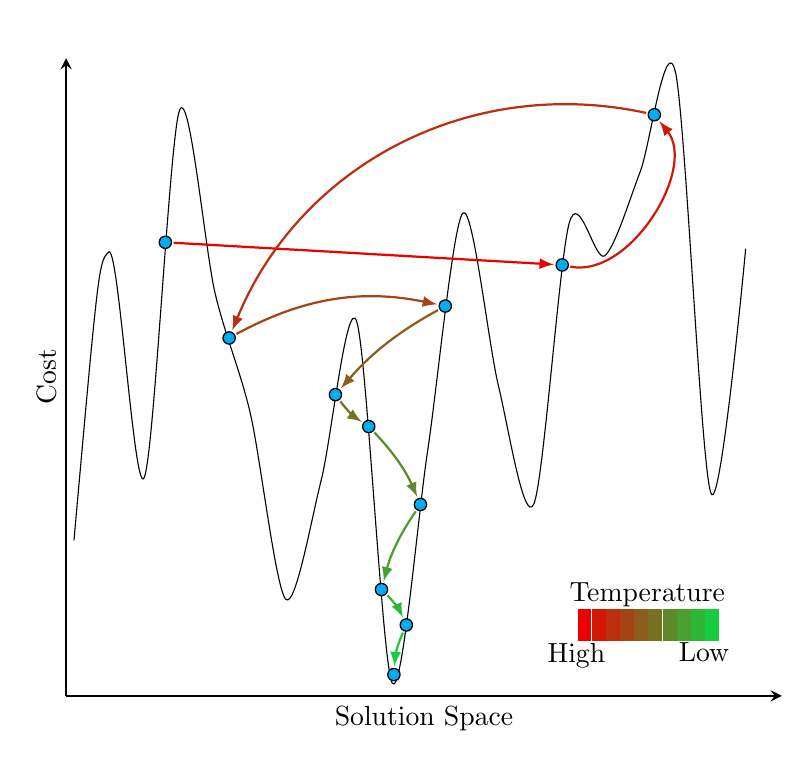
\begin{tikzpicture}
		[scale=0.9,shorten <=3pt,shorten >=3pt,>=stealth]

        \draw[thick,->,shorten <=0pt,shorten >=0pt,>=stealth] (-0.1,1) -- node[below] {Solution Space} (10,1);
        \draw[thick,->,shorten <=0pt,shorten >=0pt,>=stealth] (-0.1,1) -- node[above,sloped] {Cost} (-0.1,10);

		\draw[black,] plot [smooth] coordinates {(0,3.076)(0.5,7.263)(1,4.076)(1.5,9.263)(2,6.689)(2.5,4.981)(3,2.362)(3.5,4.046)(4,6.282)(4.5,1.183)(5,4.45)(5.5,7.813)(6,5.376)(6.5,3.708)(7,7.675)(7.5,7.209)(8,8.394)(8.5,9.791)(9,3.856)(9.5,7.428)};

        \coordinate (P1) at (1.3,7.4);
        \coordinate (P2) at (6.9,7.08);
        \coordinate (P3) at (8.2,9.2);
        \coordinate (P4) at (2.2,6.05);
        \coordinate (P5) at (5.25,6.5);
        \coordinate (P6) at (3.7,5.25);
        \coordinate (P7) at (4.17,4.8);
        \coordinate (P8) at (4.9,3.7);
        \coordinate (P9) at (4.35,2.5);
        \coordinate (P10) at (4.7,2);
        \coordinate (P11) at (4.525,1.3);
              
        \foreach \point in {P1,P2,P3,P4,P5,P6,P7,P8,P9,P10,P11}  {
            \filldraw [black] (\point) circle (2.5pt);
            \filldraw [cyan] (\point) circle (2pt);
        }

        \definecolor{C1}{RGB}{235, 0, 0}
        \definecolor{C2}{RGB}{211, 23, 7}
        \definecolor{C3}{RGB}{188, 46, 14}
        \definecolor{C4}{RGB}{164, 68, 20}
        \definecolor{C5}{RGB}{141, 91, 27}
        \definecolor{C6}{RGB}{118, 114, 34}
        \definecolor{C7}{RGB}{94, 137, 41}
        \definecolor{C8}{RGB}{71, 160, 48}
        \definecolor{C9}{RGB}{47, 182, 54}
        \definecolor{C10}{RGB}{24, 205, 61}

		\draw[-latex,color=C1,thick] (P1) to (P2);
		\draw[-latex,color=C2,thick] (P2) to[bend right=70] (P3);
		\draw[-latex,color=C3,thick] (P3) to[bend right=40] (P4);
		\draw[-latex,color=C4,thick] (P4) to[bend left=20] (P5);
		\draw[-latex,color=C5,thick] (P5) to[bend right=10] (P6);
		\draw[-latex,color=C6,thick] (P6) to[bend right=10] (P7);
		\draw[-latex,color=C7,thick] (P7) to[bend left=10] (P8);
		\draw[-latex,color=C8,thick] (P8) to[bend right=10] (P9);
		\draw[-latex,color=C9,thick] (P9) to[bend left=10] (P10);
		\draw[-latex,color=C10,thick] (P10) to[bend right=10] (P11);

        \draw[line width=4mm, color=C1] (7,2) -- ++(0.43,0);
        \draw[line width=4mm, color=C2] (7.2,2) -- ++(0.43,0);
        \draw[line width=4mm, color=C3] (7.4,2) -- ++(0.43,0);
        \draw[line width=4mm, color=C4] (7.6,2) -- ++(0.43,0);
        \draw[line width=4mm, color=C5] (7.8,2) -- ++(0.43,0);
        \draw[line width=4mm, color=C6] (8,2) -- ++(0.43,0);
        \draw[line width=4mm, color=C7] (8.2,2) -- ++(0.43,0);
        \draw[line width=4mm, color=C8] (8.4,2) -- ++(0.43,0);
        \draw[line width=4mm, color=C9] (8.6,2) -- ++(0.43,0);
        \draw[line width=4mm, color=C10] (8.8,2) -- ++(0.43,0);

        \node[above,yshift=3] at (8.1,2) {Temperature};
        \node[below,yshift=-3] at (7.1,2) {High};
        \node[below,yshift=-3] at (8.9,2) {Low};

    \end{tikzpicture}
    \caption{Iteration process of Simulated Annealing}
    \label{fig:sa}
\end{figure}

\subsection{Implementation}
For the implementation of Simulated Annealing we decided to set up a number of constants in order to be able to tweak the parameters of the 
method in input. Fixed parameters can work fine for instances of similar magnitude, but to allow for a good execution for both large and small 
instances we thought this was the best approach. The parameteres we are talking are:

\begin{enumerate}
    \item SAME\_TEMP\_MOVES\_THRESHOLD: Number of moves to perform before reducing the temperature.
    \item TEMPERATURE\_MULTIPLIER: Factor by which the temperature is multiplied to decrease it; should be slightly less than 1.
    \item STOP\_TEMP: Temperature at which SA stops and runs a 2-opt algorithm for further optimization.
    \item MAX\_TRIES\_FUNC(n): Function to determine the maximum number of move attempts before increasing the temperature.
    \item USE\_RATIO\_ACCEPTANCE: A macro to toggle the use of ratio-based acceptance criteria.
\end{enumerate}


The execution of this metaheuristic is managed by the function SimulatedAnnealing, that mainly sets up the desired number of threads and launches them 
on the function runSimulatedAnnealing. 
The actual algorithm is then executed parallely within each thread until the time limit is reached. During this time we perform moves up to what we 
specified on STOP\_TEMP, then we will launch the 2-opt metaheuristic to further refine the solution within its space. 
After a certain amount of non-improving iterations, we restart the method from the best solution found so far, which we are keeping track at all 
times and is accessible by the use of a mutex by all threads. This is to fully use the time provided in the time limit, and to give the method more chances to escape a local minima.

\subsection{Performance}

\begin{figure}[H]
	\centering
	\begin{tikzpicture}
        \begin{axis}[
            xlabel={Improvement Ratio},     % AXIS NAME
            %ylabel={Iterations/s Ratio},   % AXIS NAME
            xmin=1, xmax=1.08,       % AXIS LIMITS
            ymin=0, ymax=69,        % AXIS LIMITS
            xtick={},
            xticklabel style={/pgf/number format/fixed,/pgf/number format/precision=4},
            ytick=\empty,
            legend style={at={(0.98,0.02)},anchor=south east,legend columns=1}, %MOVE LEGEND HERE
			legend cell align={left},
            %ymajorgrids=true,
            xmajorgrids=true,
            grid style=dashed,
        ]
        
        \addplot[Blue,mark=square,mark size=1.5] table[x=improve3, y=idx, col sep=semicolon] {csv/annealing.csv}; 
        \addplot[Red,mark=o,mark size=1.5] table[x=improve6, y=idx, col sep=semicolon] {csv/annealing.csv};
        \addplot[Green,mark=triangle,mark size=1.5] table[x=improve9, y=idx, col sep=semicolon] {csv/annealing.csv};
        \addplot[Purple,mark=star,mark size=1.5] table[x=aimprove3, y=idx, col sep=semicolon] {csv/annealing.csv};
        \addplot[Dandelion,mark=otimes,mark size=1.5] table[x=aimprove6, y=idx, col sep=semicolon] {csv/annealing.csv};
        \addplot[Black,mark=diamond,mark size=1.5] table[x=aimprove9, y=idx, col sep=semicolon] {csv/annealing.csv};
        \addlegendentry{Temp = 3}
        \addlegendentry{Temp = 6}
        \addlegendentry{Temp = 9}
        \addlegendentry{Temp = 3 (alt acceptance)}
        \addlegendentry{Temp = 6 (alt acceptance)}
        \addlegendentry{Temp = 9 (alt acceptance)}
            
        \end{axis}
    \end{tikzpicture}
	\caption{Performance comparison between different Annealing configurations in terms of $\frac{final\_cost}{start\_cost}$ (Higher is better)}
    \label{fig:annealingParmTune}
\end{figure}

\begin{figure}[H]
	\centering
	\begin{tikzpicture}
        \begin{axis}[
            ylabel={Iterations/s Ratio},     % AXIS NAME
            xlabel={Sorted instances},   % AXIS NAME
            xmin=0, xmax=69,       % AXIS LIMITS
            ymin=1, ymax=2.5,        % AXIS LIMITS
            ytick={},
            xtick=\empty,
            legend style={at={(0.02,0.98)},anchor=north west,,legend columns=1}, %MOVE LEGEND HERE
			legend cell align={left},
            ymajorgrids=true,
            %xmajorgrids=true,
            grid style=dashed,
        ]
        
        
        \addplot[Blue,mark=square,mark size=1.5] table[y=iter3, x=idx, col sep=semicolon] {csv/annealing.csv}; 
        \addplot[Red,mark=o,mark size=1.5] table[y=iter6, x=idx, col sep=semicolon] {csv/annealing.csv};
        \addplot[Green,mark=triangle,mark size=1.5] table[y=iter9, x=idx, col sep=semicolon] {csv/annealing.csv};
        \addplot[Purple,mark=star,mark size=1.5] table[y=aiter3, x=idx, col sep=semicolon] {csv/annealing.csv};
        \addplot[Dandelion,mark=otimes,mark size=1.5] table[y=aiter6, x=idx, col sep=semicolon] {csv/annealing.csv};
        \addplot[Black,mark=diamond,mark size=1.5] table[y=aiter9, x=idx, col sep=semicolon] {csv/annealing.csv};
        \addlegendentry{Temp = 3}
        \addlegendentry{Temp = 6}
        \addlegendentry{Temp = 9}
        \addlegendentry{Temp = 3 (alt acceptance)}
        \addlegendentry{Temp = 6 (alt acceptance)}
        \addlegendentry{Temp = 9 (alt acceptance)}
            
        \end{axis}
    \end{tikzpicture}
	\caption{Comparison between Simulated Annealing parameters in speed}
    \label{fig:annealingIters}
\end{figure}

There does not seems to be any favorable configuration (next graph uses temp=6 data (no alt edge acceptance))

\begin{figure}[H]
	\centering
	\begin{tikzpicture}
        \begin{axis}[
            xlabel={Cost Ratio},     % AXIS NAME
            %ylabel={Iterations/s Ratio},   % AXIS NAME
            xmin=1, xmax=1.082,       % AXIS LIMITS
            ymin=0, ymax=69,        % AXIS LIMITS
            xtick={},
            ytick=\empty,
            legend style={at={(0.98,0.02)},anchor=south east,legend columns=1}, %MOVE LEGEND HERE
			legend cell align={left},
            %ymajorgrids=true,
            xmajorgrids=true,
            grid style=dashed,
        ]
        
        \addplot[Blue,mark=square,mark size=1.5] table[x=startcost,y=idx, col sep=semicolon] {csv/annealing.csv}; 
        \addplot[Red,mark=o,mark size=1.5] table[x=finalcost,y=idx, col sep=semicolon] {csv/annealing.csv};
        \addplot[Green,mark=triangle,mark size=1.5] table[x=optimalcost,y=idx, col sep=semicolon] {csv/annealing.csv}; 
        \addlegendentry{Initial Cost} 
        \addlegendentry{Final Cost}
        \addlegendentry{Optimal Cost}
            
        \end{axis}
    \end{tikzpicture}
	\caption{Overall Performance of Simulated Annealing}
    \label{fig:annealingCost}
\end{figure}

\section{Genetic}
\subsection{Implementation}
In a similar fashion of the algorithms previously presented, for the Genetic Algorithm we also have a main method, GeneticAlgorithm, that is in 
charge of managing the creation and synchronization of the various threads. The actual algorithm is performed then within each thread by the function runGenetic.
A series macros are used throughout the code to configure the genetic algorithm's behavior without hardcoding values. For example, the population 
size and the number of genetic operations (crossover, mutation, reintroduction) are dynamically calculated based on the instance parameters using 
POPULATION\_SIZE, CROSSOVER\_AMOUNT, MUTATION\_AMOUNT and REINTRO\_AMOUNT. 

\subsection{Performance}

\begin{itemize}
    \item \textbf{Config 1}: Population = 50, Crossover = 10, Mutation = 10, Reintro =  5
    \item \textbf{Config 1}: Population = 50, Crossover = 20, Mutation = 20, Reintro =  5
    \item \textbf{Config 1}: Population = 100, Crossover = 50, Mutation = 20, Reintro = 20
    \item \textbf{Config 1}: Population = 100, Crossover = 20, Mutation = 50, Reintro = 20
    \item \textbf{Config 1}: Population = 100, Crossover = 40, Mutation = 40, Reintro = 10
\end{itemize}

\begin{figure}[H]
	\centering
	\begin{tikzpicture}
        \begin{axis}[
            xlabel={Cost Ratio},     % AXIS NAME
            %ylabel={Iterations/s Ratio},   % AXIS NAME
            xmin=1, xmax=2.7,       % AXIS LIMITS
            ymin=0, ymax=42,        % AXIS LIMITS
            xtick={},
            xticklabel style={/pgf/number format/fixed,/pgf/number format/precision=4},
            ytick=\empty,
            legend style={at={(0.98,0.02)},anchor=south east,legend columns=1}, %MOVE LEGEND HERE
			legend cell align={left},
            %ymajorgrids=true,
            xmajorgrids=true,
            grid style=dashed,
        ]
        
        \addplot[Blue,mark=square,mark size=1.5] table[x=cost_50_10_10_5, y=idx, col sep=semicolon] {csv/genetic.csv}; 
        \addplot[Red,mark=o,mark size=1.5] table[x=cost_50_20_20_5, y=idx, col sep=semicolon] {csv/genetic.csv};
        \addplot[Green,mark=triangle,mark size=1.5] table[x=cost_100_50_20_20, y=idx, col sep=semicolon] {csv/genetic.csv};
        \addplot[Purple,mark=star,mark size=1.5] table[x=cost_100_20_50_20, y=idx, col sep=semicolon] {csv/genetic.csv};
        \addplot[Dandelion,mark=otimes,mark size=1.5] table[x=cost_100_40_40_10, y=idx, col sep=semicolon] {csv/genetic.csv};
        \addlegendentry{Config 1}
        \addlegendentry{Config 2}
        \addlegendentry{Config 3}
        \addlegendentry{Config 4}
        \addlegendentry{Config 5}
            
        \end{axis}
    \end{tikzpicture}
	\caption{Performance comparison between different Genetic configurations}
    \label{fig:geneticParmTune}
\end{figure}

\begin{figure}[H]
	\centering
	\begin{tikzpicture}
        \begin{axis}[
            ylabel={Iterations/s Ratio},     % AXIS NAME
            xlabel={Sorted instances},   % AXIS NAME
            xmin=0, xmax=42,       % AXIS LIMITS
            ymin=1, ymax=8,        % AXIS LIMITS
            ytick={},
            xtick=\empty,
            legend style={at={(0.02,0.98)},anchor=north west,,legend columns=1}, %MOVE LEGEND HERE
			legend cell align={left},
            ymajorgrids=true,
            %xmajorgrids=true,
            grid style=dashed,
        ]
        
        
        \addplot[Blue,mark=square,mark size=1.5] table[y=iter_50_10_10_5, x=idx, col sep=semicolon] {csv/genetic.csv}; 
        \addplot[Red,mark=o,mark size=1.5] table[y=iter_50_20_20_5, x=idx, col sep=semicolon] {csv/genetic.csv};
        \addplot[Green,mark=triangle,mark size=1.5] table[y=iter_100_50_20_20, x=idx, col sep=semicolon] {csv/genetic.csv};
        \addplot[Purple,mark=star,mark size=1.5] table[y=iter_100_20_50_20, x=idx, col sep=semicolon] {csv/genetic.csv};
        \addplot[Dandelion,mark=otimes,mark size=1.5] table[y=iter_100_40_40_10, x=idx, col sep=semicolon] {csv/genetic.csv};
        \addlegendentry{Config 1}
        \addlegendentry{Config 2}
        \addlegendentry{Config 3}
        \addlegendentry{Config 4}
        \addlegendentry{Config 5}
            
        \end{axis}
    \end{tikzpicture}
	\caption{Comparison between Genetic configurations in speed}
    \label{fig:geneticIters}
\end{figure}

\begin{figure}[H]
	\centering
	\begin{tikzpicture}
        \begin{axis}[
            xlabel={Cost Ratio},     % AXIS NAME
            %ylabel={Iterations/s Ratio},   % AXIS NAME
            xmin=1, xmax=17,       % AXIS LIMITS
            ymin=0, ymax=42,        % AXIS LIMITS
            xtick={},
            ytick=\empty,
            legend style={at={(0.98,0.02)},anchor=south east,legend columns=1}, %MOVE LEGEND HERE
			legend cell align={left},
            %ymajorgrids=true,
            xmajorgrids=true,
            grid style=dashed,
        ]
        
        \addplot[Red,mark=o,mark size=1.5] table[x=finalcost,y=idx, col sep=semicolon] {csv/genetic.csv}; 
        \addplot[Green,mark=triangle,mark size=1.5] table[x=optimalcost,y=idx, col sep=semicolon] {csv/genetic.csv};
        \addlegendentry{Final Cost}
        \addlegendentry{Optimal Cost}
            
        \end{axis}
    \end{tikzpicture}
	\caption{Overall Performance of Genetic}
    \label{fig:geneticCost}
\end{figure}

\section{Comparison}

\begin{figure}[H]
	\centering
	\begin{tikzpicture}
        \begin{axis}[
            xlabel={Cost Ratio},     % AXIS NAME
            %ylabel={Iterations/s Ratio},   % AXIS NAME
            xmin=1, xmax=1.05,       % AXIS LIMITS
            ymin=0, ymax=74,        % AXIS LIMITS
            xtick={},
            xticklabel style={/pgf/number format/fixed,/pgf/number format/precision=4},
            ytick=\empty,
            legend style={at={(0.98,0.02)},anchor=south east,legend columns=1}, %MOVE LEGEND HERE
			legend cell align={left},
            %ymajorgrids=true,
            xmajorgrids=true,
            grid style=dashed,
        ]
        
        \addplot[Blue,mark=square,mark size=1.5] table[x=tabu_1, y=idx, col sep=semicolon] {csv/cmp_metaheuristics.csv}; 
        \addplot[Red,mark=o,mark size=1.5] table[x=vns_5-10, y=idx, col sep=semicolon] {csv/cmp_metaheuristics.csv};
        \addplot[Green,mark=triangle,mark size=1.5] table[x=annealing_std6, y=annealing_idx, col sep=semicolon] {csv/cmp_metaheuristics.csv};
        % \addplot[Purple,mark=star,mark size=1.5] table[x=genetic, y=genetic_idx, col sep=semicolon] {csv/cmp_metaheuristics.csv};
        \addlegendentry{tabu}
        \addlegendentry{VNS}
        \addlegendentry{Annealing}
        % \addlegendentry{Genetic}
            
        \end{axis}
    \end{tikzpicture}
	\caption{Comparsion between all metaheuristics with best parameters found}
    \label{fig:metacmp}
\end{figure}

\chapter{Cplex}

CPLEX is a high-performance optimization software developed by IBM that specializes in solving mathematical programming problems, including linear programming, mixed-integer programming, and quadratic programming, among others. It is one of the most widely used commercial solvers for solving complex optimization problems in various industries and academic research.

CPLEX provides a comprehensive suite of algorithms and techniques to efficiently solve optimization problems of varying sizes and complexities. It employs state-of-the-art optimization algorithms, such as the primal-dual interior point method for linear programming and branch-and-bound algorithms for mixed-integer programming, to find high-quality solutions within reasonable timeframes. 

One of the key features of CPLEX is its ability to handle large-scale optimization problems efficiently. It incorporates advanced preprocessing techniques, presolve routines, and cutting-plane algorithms to reduce problem size and improve solution quality. Additionally, CPLEX offers parallel computing capabilities, leveraging multiple CPU cores and distributed computing environments to accelerate the solution process for large-scale problems.

Overall, CPLEX is a powerful optimization tool that enables users to model, solve, and analyze complex optimization problems across diverse domains, including operations research, logistics, supply chain management, finance, and engineering. Its robust performance, scalability, and versatility make it a valuable asset for researchers, practitioners, and organizations seeking to optimize their decision-making processes.

CPLEX is useful for solving the TSP due to its efficient solver, scalability for large instances, support for Mixed-Integer Programming formulations commonly used for TSP, integration with programming languages like Python, and parallel computing capabilities, enabling faster solution times for complex TSP instances.



\section{Integer Linear Programming Formulation of TSP}

In order to use CPLEX to solve the TSP we first need to define an integer linear programming (ILP) model for it. \\
Let's denote the graph as $G=(V,E)$, where $V$ represents the set of nodes (vertices) and $E$ represents the set of edges.
Let $n$ be the number of nodes in the graph, and let $c_{ij}$ represent the cost (weight) of traveling from node $i$ to node $j$ in the graph $G$. If there is no direct edge between nodes $i$ and $j$, we can set $c_{ij}$ to a large value to indicate that traveling between these nodes is not allowed. \\
A possbile ILP model can be formulated using the following decision variable
\begin{align*}
	& x_{ij} = 
	\begin{cases}
		1, & \text{if edge } (i,j)\in E \text{ is chosen in the optimal circuit}\\
		0, & \text{otherwise}
	\end{cases}
\end{align*}
Using fact that in a TSP solution each node has degree equal to two we obtain:
\begin{align}
	\text{min} &\sum\limits_{(i,j)\in E} c_{ij} \cdot x_{ij} \tag{1.1}\label{eq:1.1} \\
	&\sum\limits_{\:\;\;j=1\:\;\;}^{n} x_{ij} = 2 \quad \text{for } i = 1,2,\ldots,n \tag{1.2}\label{eq:1.2} \\
	&\sum\limits_{(i,j)\in C} x_{ij} \leq |C| - 1 \quad \forall \; C: C \text{ is a subtour of } G \tag{1.3}\label{eq:1.3}
\end{align}
where equation \eqref{eq:1.1} is the total cost of the circuit, constraints \eqref{eq:1.2} are the degree constraints and \eqref{eq:1.3} are the Subtour Elimination Constraints(SEC). Counting the number of constraints we have $n$ constraints from \eqref{eq:1.2} and an exponential amount from \eqref{eq:1.3}. A number of constraints that big makes in practice the problem much harder to resolve, so a common workaround also used in the following algorithms is to ignore SEC and add only the ones that are violated each time cplex returns a feasible solution.

\section{Initialization of CPLEX}

In order to use CPLEX we must initialize the problem first, that means write the TSP according to CPLEX standards. To do this we start with an empty problem and then proceed to add all necessary elements to represent the ILP formulation described previously.

In order to create the empty problem one must simply call the functions \textbf{CPXopenCPLEX} to initialize CPLEX itself and \textbf{CPXcreateprob} to create the problem itself.
Having created the problem it must be populated with variables(columns) and constratints(rows). Variables $x_{ij}$ are added through the function \textbf{CPXnewcols} either in a sequential way(one at a time) or all at the same time by allocating the needed memory and passing cplex all variables by means of arrays, which can be a tedious process except some cases in which it may be easier that way(for example if the data in the instance is saved in a similar way).
The next step is to add constraints. As discussed before it's more efficient to only add constraints specified by \eqref{eq:1.2} without any SEC constraints \eqref{eq:1.3}. The procedure is very similar to the one to add variables: function \textbf{CPXaddrows} can add multiple constraints(rows) at once or one at a time like \textbf{CPXnewcols} and like \textbf{CPXnewcols} the easier way is the sequential one.
This procedure is sumarized in the algorithm below

\begin{algorithm}[H]
	\TitleOfAlgo{\textbf{CPLEX initialization}}
    \SetKwInOut{Input}{input}
    \SetKwInOut{Output}{output}
    \Input{Graph $G(V,E)$ fully connected \newline$c_{ij}=$ cost of $edge(i,j) \in |E|$ }
	\Output{Instance initialized in CPLEX}
	\vspace{2mm}
	Create empty CPLEX linear problem $p$\\
	\ForEach{edge $e_{ij} \in E$}{
		Add binary variable $x_{i,j}$ with associated cost $c_{ij}$ to $p$\\
	}
	\ForEach{$v \in \{1, \dots ,|V|\}$}{
        $s_v=\sum\limits_{(i,j) \in E} y_{ij}$ where $y_{ij} = 1 \iff i=v$ or $j=v$; otherwise $y_{i,j} = 0$\\
        Add constraint $s_v \leq 2$ to $p$\\
	}
	\Return{$p$}
\end{algorithm}

\section{CPLEX edge representation}

This section describes how to extract and convert a solution obtained using CPLEX into a more compact way. 
By itself CPLEX returns as solution of the TSP an array with the full set of variables $x_{ij}$ which is a bit tedious to read and to use custom functions on top.
To improve this one can convert the solution to a \textit{successors} array. 

\begin{function}[H]
	\TitleOfAlgo{\textbf{xpos}}
    \SetKwInOut{Input}{input}
    \SetKwInOut{Output}{output}
    \Input{$i$, $j$, $|V|$}
	\Output{position of $edge(i,j)$ in CPLEX notation}
	\vspace{2mm}
	\If{$i = j$}{ Error\; }
	\If{$i > j$}{ $i \Leftrightarrow j$\; }
	\Return{$i * |V| + j - ((i + 1) * (i + 2)) / 2$}
\end{function}

\chapter{Exact Solvers}

\section{Benders}

\subsection{Patching Heuristic}

\section{Branch \& Cut}

\subsection{Solution Posting}

\subsection{Concorde \& User Cuts}

\chapter{Matheuristics}

\section{Hard Fixing}

\section{Local Branching}





\begin{thebibliography}{9}
	\bibitem{tsplib}
	\url{http://comopt.ifi.uni-heidelberg.de/software/TSPLIB95/}

	\bibitem{newtonMethod}
	\url{https://en.wikipedia.org/wiki/Newton%27s_method}

	\bibitem{avxWikipedia}
	\url{https://en.wikipedia.org/wiki/Advanced_Vector_Extensions}

	\bibitem{vnsWikipedia}
	\url{https://en.wikipedia.org/wiki/Variable_neighborhood_search}

\end{thebibliography}

\end{document}

